% ============================================================
%  Informe final del proyecto
%  Equipo de Ensayos de Seguridad Eléctrica Portátil
%  Autora: Valentina Ferrini
%
%  Compilar con: latexmk -pdf main.tex   (o pdflatex + biber + pdflatex x2)
%  Estructura: este archivo arma el documento; cada sección está en /sections.
% ============================================================
\documentclass[a4paper,12pt]{article}

% --- Codificación e idioma ---
\usepackage[utf8]{inputenc}
\usepackage[T1]{fontenc}
\usepackage{lmodern}
\usepackage[spanish,es-tabla]{babel}

% --- Página ---
\usepackage[margin=2.5cm]{geometry}

% --- Matemática, unidades y tablas ---
\usepackage{amsmath}
\usepackage{amssymb}
\usepackage{siunitx}
\sisetup{output-decimal-marker={,}, group-minimum-digits=4, per-mode=symbol}
\DeclareSIUnit\baud{Bd}
\DeclareSIUnit\USD{USD}
\usepackage{booktabs}
\usepackage{multirow}
\usepackage{longtable}
\usepackage{array}
\usepackage{tabularx}
\usepackage[table]{xcolor}

% --- Figuras ---
\usepackage{graphicx}
\usepackage{float}
\usepackage{caption}
\usepackage{subcaption}
\graphicspath{{figuras/}{evidencia_banco/fotos/}}
% Las figuras y tablas no pasan a la sección siguiente
\usepackage[section]{placeins}

% Índice: espacio para números de sección de dos dígitos
\usepackage{tocloft}
\setlength{\cftsecnumwidth}{2.2em}
\setlength{\cftsubsecnumwidth}{3.2em}
\setlength{\cftsubsubsecnumwidth}{4.2em}
\renewcommand{\cftsecleader}{\cftdotfill{\cftdotsep}}

% --- Títulos de párrafo en bloque ---
\usepackage{titlesec}
\titleformat{\paragraph}[block]{\normalfont\normalsize\bfseries}{}{0em}{}
\titlespacing*{\paragraph}{0pt}{1ex plus .2ex}{0.5ex}

% --- Anexos y referencias ---
\usepackage[title,titletoc]{appendix}
% Los anexos se titulan "Anexo" (babel en español usa "Apéndice")
\addto\captionsspanish{\renewcommand{\appendixname}{Anexo}}
\renewcommand{\appendixtocname}{Anexos}
\renewcommand{\appendixpagename}{Anexos}
\usepackage[backend=biber,style=numeric,sorting=none]{biblatex}
\addbibresource{referencias.bib}
\usepackage{csquotes}
\usepackage{xurl}
\usepackage{hyperref}
\hypersetup{colorlinks=true, linkcolor=black, citecolor=blue!50!black,
            urlcolor=blue!50!black}

% --- Macros del documento ---
% Figura que se incluye solo si el archivo existe; si no, deja un recuadro
% indicando qué imagen falta (para no romper la compilación).
\newcommand{\figuraopcional}[2]{%
  \IfFileExists{figuras/#1}{\includegraphics[width=#2]{#1}}{%
    \fbox{\parbox{#2}{\centering\vspace{1.5cm}%
      \textit{Falta la imagen \texttt{figuras/\detokenize{#1}}}\vspace{1.5cm}}}}}
% Marca visible de contenido pendiente (eliminar antes de la entrega).
\newcommand{\pendiente}[1]{\textcolor{red}{\textbf{[PENDIENTE: #1]}}}

\title{Equipo de Ensayos de Seguridad Eléctrica Portátil\\[0.5em]
       \large Informe final del Trabajo Final de Grado}
\author{Valentina Ferrini}
\date{Noviembre 2026}

\begin{document}

\maketitle
\thispagestyle{empty}
\newpage

% ============================================================
%  Resumen
% ============================================================
\begin{center}
    \textbf{\huge Resumen}
\end{center}
\vspace{1cm}

En la actualidad, la seguridad eléctrica de los equipos de uso doméstico y
comercial constituye un requisito fundamental para su comercialización. Sin
embargo, los métodos tradicionales de ensayo, basados en la intervención manual
del operario, pueden generar variaciones en los resultados, extender los tiempos
de prueba y aumentar los riesgos para el personal y los dispositivos bajo
evaluación.

Este trabajo presenta el desarrollo de un sistema integral, conformado por un
dispositivo de ensayos y una interfaz de software, destinado a verificar en final
de línea el cumplimiento de la norma IEC~60335-1 en aparatos electrodomésticos:
consumo, corriente de fuga activa y pasiva, resistencia de puesta a tierra y
rigidez dieléctrica. El dispositivo se basa en un microcontrolador ESP32 que lee
medidores PZEM-004T y en relés y contactores que conmutan los circuitos de ensayo;
la interfaz, desarrollada en Python y PyQt5, configura y secuencia los ensayos,
emite el veredicto, registra los resultados en una base de datos y los exporta.

Durante el desarrollo se alinearon los criterios de aprobación con los ensayos de
rutina del Anexo~A y las cláusulas~10 y~16 de la norma, se escribió el firmware
del microcontrolador y se integró y verificó el sistema en un banco de pruebas
real. El software se probó con hardware real en dos equipos: en un equipo
completo provisto por SYGlab y esquematizado por la autora, donde su versión
inicial ejecutó los ensayos de seguridad y registró 86 verificaciones con
patrones, y en un prototipo propio, donde la versión final se verificó de punta a
punta en el ensayo de consumo sobre cargas reales. Los cambios de la versión
final en los ensayos de fuga, puesta a tierra y rigidez dieléctrica se
verificaron con hardware simulado. Se documentan además las
dificultades encontradas ---entre ellas un problema de compatibilidad
electromagnética en el control de los relés--- y las soluciones adoptadas.

\newpage


\tableofcontents
\newpage

% ============================================================
%  Introducción y objeto
% ============================================================
\section{Introducción}
\label{sec:introduccion}

En la industria de la fabricación de dispositivos eléctricos, la seguridad
eléctrica es un aspecto crítico para garantizar la protección de los usuarios.
La norma IEC~60335 establece los ensayos de seguridad que deben cumplir los
aparatos electrodomésticos y similares antes de su comercialización
\cite{iec60335}. Los métodos tradicionales de prueba, que dependen en gran medida
de la intervención manual del operario, pueden dar lugar a variaciones en los
resultados, prolongar los tiempos de prueba y aumentar los riesgos tanto para el
personal como para los dispositivos bajo evaluación.

El presente informe describe el diseño, la construcción y la verificación de un
equipo portátil y semiautomatizado para ejecutar esos ensayos en final de línea,
los resultados obtenidos en el banco de pruebas y las conclusiones del trabajo.

\section{Objeto}
\label{sec:objeto}

La seguridad eléctrica se ha convertido en un pilar indispensable para la
confiabilidad y comercialización de los equipos de uso doméstico e industrial. En
este contexto, surge la necesidad de innovar en los procesos de verificación,
superando las limitaciones de los métodos tradicionales que dependen en gran
medida de la intervención humana. Este proyecto tiene por objeto el diseño y la
construcción de un dispositivo semiautomatizado capaz de ejecutar, con precisión
y repetibilidad, las principales pruebas de seguridad definidas en la norma
internacional IEC~60335 ---rigidez dieléctrica, continuidad de tierra, medición
de corrientes de fuga y consumo---, garantizando así un control de calidad más
eficiente y seguro.

\vspace{0.3cm}\noindent El desarrollo se complementa con una interfaz de software
que integra los distintos subsistemas, procesa los datos obtenidos y facilita la
interacción con el operario. De este modo, se busca no solo reducir los tiempos de
prueba y minimizar los riesgos, sino también aportar una herramienta que eleve los
estándares de confiabilidad y trazabilidad en el control de calidad de productos
eléctricos.

% ============================================================
%  Estado del arte y normativa
% ============================================================
\section{Estado del arte y normativas aplicables}
\label{sec:estado_arte}

\subsection{Panorama de los ensayos de seguridad eléctrica en la industria}

La seguridad eléctrica es un aspecto fundamental en la fabricación de productos
eléctricos y electrónicos, ya que garantiza tanto la integridad de los equipos como
la protección de los usuarios. Los ensayos de seguridad, que incluyen pruebas de
rigidez dieléctrica, continuidad de tierra y corriente de fuga, son requisitos
obligatorios para la certificación de productos en diversos mercados.
Tradicionalmente, estos ensayos se han realizado de manera manual, lo que puede dar
lugar a variabilidad en los resultados, prolongar los tiempos de prueba y generar
riesgos tanto para el personal como para los productos. Por esta razón, ha surgido
un creciente interés en la automatización de estos procesos, con el objetivo de
mejorar la precisión, la reproducibilidad y la eficiencia operativa, además de
garantizar la trazabilidad y un historial completo de las pruebas realizadas.
Existen en el mercado equipos comerciales que integran estos ensayos, como la
línea EFE Plus \cite{efeplus} o los equipos de Insatec \cite{insatec}, y
laboratorios que los ofrecen como servicio \cite{labconsultar}.

\subsection{Los ensayos de seguridad eléctrica más comunes}
\begin{itemize}
    \item \textbf{Rigidez dieléctrica (tensión resistida):} se aplica una tensión
          elevada entre las partes activas y las partes accesibles para verificar
          el aislamiento.
    \item \textbf{Continuidad de tierra:} verifica que la resistencia entre el
          borne de tierra y las partes metálicas accesibles sea baja.
    \item \textbf{Corriente de fuga:} asegura que las corrientes indeseadas hacia
          las partes accesibles estén dentro de los límites permitidos.
    \item \textbf{Consumo:} verifica que la potencia o la corriente absorbida no se
          aparte del valor nominal marcado más allá de la tolerancia admitida.
\end{itemize}

\subsection{Métodos tradicionales y su grado de automatización}

El proceso de prueba tradicional requiere intervención manual del operario y la
disposición del instrumental junto con personal capacitado, lo cual puede
producir variaciones en los resultados, demoras en las pruebas y posibles riesgos
para el personal, los instrumentos y los productos.

\subsection{Normativa aplicable}
\label{subsec:normativa}

La norma IEC~60335 establece requisitos de seguridad para aparatos eléctricos de
uso doméstico y aplicaciones comerciales de baja tensión. La parte~1
(IEC~60335-1) contiene los requisitos generales aplicables a todos los aparatos
comprendidos en la norma; en este trabajo se toma como referencia la
edición~4.1 \cite{iec60335}. La norma distingue los \textbf{ensayos de tipo}
(cláusulas~10 a~32), que certifican un diseño sobre muestras representativas, de
los \textbf{ensayos de rutina} (Anexo~A), que se aplican a cada unidad producida.
Por ser un equipo de final de línea, el sistema adopta los ensayos de rutina del
Anexo~A donde existen.

Otras normas de referencia contextual son:
\begin{itemize}
    \item \textbf{IEC~61010:} seguridad de equipos de medida, control y laboratorio
          \cite{iec61010}.
    \item \textbf{IEC~60950 / IEC~62368:} seguridad de equipos de tecnología de la
          información y audio/video \cite{iec62368}.
    \item \textbf{UL~60950 / UL~62368:} equivalentes para el mercado de EE.\,UU.
    \item \textbf{IRAM~2435:} norma argentina de referencia \cite{iram2435}.
    \item \textbf{ISO/IEC~17025:} competencia de laboratorios de ensayo y
          calibración \cite{iso17025}.
    \item \textbf{IEC~60990:} métodos de medición de la corriente de contacto y de
          la corriente del conductor de protección \cite{iec60990}.
\end{itemize}

\noindent Para el alcance de este proyecto se aplica la IEC~60335 y sus anexos.
La certificación del equipo ante el Organismo Argentino de Acreditación (OAA) u
otros organismos queda fuera del alcance, aunque el diseño se orienta al
cumplimiento normativo.

% ============================================================
%  Motivación
% ============================================================
\section{Motivación y planteo del problema}
\label{sec:motivacion}

\subsection{La necesidad de un sistema automatizado}

Los ensayos de seguridad eléctrica son esenciales para certificar y comercializar
productos eléctricos. Los métodos manuales presentan limitaciones como la
variabilidad de los resultados, mayores tiempos de prueba, riesgos operativos y
errores en la toma de datos. El desarrollo de un sistema automatizado de principio
a fin para realizar estos ensayos tiene como objetivo mejorar la precisión,
reducir la intervención humana y optimizar el tiempo de evaluación.

\subsection{Beneficios esperados}
\begin{itemize}
    \item Mayor precisión y repetibilidad en los resultados.
    \item Reducción de tiempos mediante la automatización de la secuencia de
          ensayos.
    \item Historial digital de los ensayos, que asegura la trazabilidad,
          facilita el análisis, respalda la certificación de productos y sirve de
          documentación en auditorías.
    \item Mayor cumplimiento normativo, al aplicar de forma sistemática los
          criterios de la norma.
\end{itemize}

% ============================================================
%  Alcance del proyecto
% ============================================================
\section{Alcance del proyecto}
\label{sec:alcance}

El proyecto contempla el diseño y la construcción de un sistema integral de
ensayos de seguridad eléctrica, compuesto por un dispositivo físico y una interfaz
de software, destinado a verificar el cumplimiento de la norma IEC~60335. El
alcance abarca tanto los aspectos funcionales como no funcionales, además de las
restricciones, supuestos y riesgos asociados al desarrollo.

\subsection{Requerimientos funcionales y no funcionales}

\subsubsection{Requerimientos funcionales}
\begin{itemize}
    \item Ejecución de los ensayos de consumo, rigidez dieléctrica, continuidad de
          tierra y corrientes de fuga (activa y pasiva).
    \item Automatización de la configuración, conmutación, adquisición y
          procesamiento de datos.
    \item Generación de reportes digitales trazables y exportables.
    \item Interfaz gráfica intuitiva para la configuración y supervisión de
          ensayos.
\end{itemize}

\subsubsection{Requerimientos no funcionales}
\begin{itemize}
    \item \textbf{Confiabilidad:} resultados reproducibles con un error acotado
          respecto de los límites de la norma IEC~60335.
    \item \textbf{Seguridad:} protecciones contra sobrecargas, aislamiento
          adecuado, alarmas y comportamiento seguro ante fallas.
    \item \textbf{Usabilidad:} intervención mínima del operario y curva de
          aprendizaje baja.
    \item \textbf{Escalabilidad:} posibilidad de incorporar nuevos ensayos o
          adaptarse a modificaciones normativas.
    \item \textbf{Mantenibilidad:} arquitectura modular de hardware y software que
          facilite la reparación, actualización y extensión del sistema.
\end{itemize}

\subsection{Restricciones}
\begin{itemize}
    \item Presupuesto limitado para la construcción del prototipo y la adquisición
          de componentes.
    \item Disponibilidad restringida de equipamiento especializado para
          calibración y validación.
    \item Tiempo máximo de ejecución establecido en el cronograma del proyecto
          (Anexo~\ref{anx:cronograma}).
    \item Cumplimiento de las normativas IEC aplicables.
\end{itemize}

\subsection{Supuestos}
\begin{itemize}
    \item Se contará con un laboratorio equipado para la ejecución de ensayos de
          validación.
    \item Los componentes electrónicos necesarios estarán disponibles en el
          mercado local o mediante proveedores confiables.
    \item El personal que utilice el sistema tendrá capacitación básica en
          seguridad eléctrica y operación de equipos de ensayo.
\end{itemize}

\subsection{Riesgos y mitigación}
\begin{itemize}
    \item \textbf{Retrasos en la adquisición de componentes:} pueden comprometer el
          cronograma. Se mitigan identificando tempranamente proveedores
          alternativos.
    \item \textbf{Fallas en la calibración o en la validación del sistema:} podrían
          impedir la aceptación del proyecto. Se mitigan con pruebas piloto e
          intercomparaciones con equipos certificados.
    \item \textbf{Limitaciones presupuestarias:} aumentos de costos podrían superar
          lo estimado. Se mitigan con un margen de contingencia.
    \item \textbf{Problemas de integración entre hardware y software:} se mitigan
          con un desarrollo incremental y pruebas de integración tempranas.
\end{itemize}

\subsection{Aspectos fuera del alcance}

El proyecto se centra en el diseño, construcción y verificación de un sistema
semiautomatizado de ensayos eléctricos orientado a la norma IEC~60335. No forman
parte del alcance:
\begin{itemize}
    \item La certificación oficial del equipo ante organismos nacionales o
          internacionales (OAA, IEC, UL, entre otros), aunque el diseño se orienta
          a cumplir con dichas normativas.
    \item Ensayos no contemplados en la IEC~60335, como medición de armónicos,
          pruebas de sobrecarga o compatibilidad electromagnética.
    \item La fabricación industrial en serie del dispositivo; el trabajo se limita
          a un prototipo funcional.
    \item El mantenimiento y soporte a largo plazo del sistema.
    \item La integración con sistemas de gestión externos (ERP, MES, etc.), más
          allá del almacenamiento local y la exportación de datos.
\end{itemize}

% ============================================================
%  Requisitos del sistema
% ============================================================
\section{Requisitos del sistema a desarrollar}
\label{sec:requisitos}

\subsection{Hardware}
\label{subsec:requisitos_hw}

El subsistema de hardware constituye el núcleo físico del equipo. Su función es
ejecutar, de forma controlada y repetible, los procedimientos de medición
definidos por la norma IEC~60335, garantizando la seguridad del operario y la
trazabilidad de los resultados. El dispositivo debe cubrir:
\begin{itemize}
    \item Medición de consumo (tensión, corriente, potencia activa y factor de
          potencia).
    \item Medición de corriente de fuga activa y pasiva.
    \item Medición de resistencia de puesta a tierra.
    \item Ensayo de rigidez dieléctrica (tensión resistida).
    \item Conmutación automática entre los circuitos de ensayo y desconexión
          del aparato bajo ensayo (DUT).
    \item Medidas de seguridad: aislamiento entre etapas, protecciones,
          desconexión ante falla, indicadores y paro de emergencia.
\end{itemize}

\subsection{Software}
\label{subsec:requisitos_sw}

La interfaz debe abarcar:
\begin{itemize}
    \item Ejecución de los cinco ensayos, adaptando los límites a los atributos
          del producto (clase de aislamiento, tipo de aparato, cable de
          alimentación, condición de duplicación del límite de fuga).
    \item Configuración de productos y tiempos de ensayo, secuencia automática de
          ensayos, adquisición y procesamiento de datos y veredicto automático.
    \item Alarmas ante valores anormales o fallas del equipo.
    \item Registro histórico trazable y exportación de resultados.
\end{itemize}

% ============================================================
%  Metodología y desarrollo
% ============================================================
\section{Metodología y desarrollo}
\label{sec:metodologia}

El desarrollo siguió una estrategia incremental: primero se definieron los
criterios de ensayo a partir de la norma, luego se construyeron por separado el
dispositivo y la interfaz, y finalmente se integraron y verificaron en un banco de
pruebas real con cargas conocidas. Esta sección describe el diseño del hardware,
el del software y los criterios metodológicos adoptados para cada ensayo.

% ------------------------------------------------------------
\subsection{Desarrollo del hardware}
\label{subsec:metodologia_hw}
% ------------------------------------------------------------

\subsubsection{Equipo completo de referencia y prototipo propio}
\label{subsubsec:equipo_syglab}

El trabajo se apoyó en dos equipos con propósitos distintos:
\begin{itemize}
    \item \textbf{Equipo completo de referencia:} un equipo de ensayos de final de
          línea provisto por SYGlab, que realiza los ensayos de consumo,
          corriente de fuga, puesta a tierra, tensión resistida (rigidez
          dieléctrica) y corte de neutro, con la misma
          arquitectura de este proyecto: medidores PZEM, relés, contactores y
          transformadores de ensayo comandados desde una PC. El hardware fue
          provisto por SYGlab; su esquematización ---el relevamiento del
          conexionado y los esquemas de conexión de cada ensayo
          (Anexo~\ref{anx:evidencia})--- fue realizada por la autora. En ese equipo
          se ejecutó la versión inicial del software desarrollado en este
          trabajo, que luego se amplió y corrigió hasta su versión final.
    \item \textbf{Prototipo propio:} un banco armado por la autora para el ensayo
          de consumo, sobre el que se desarrolló y verificó de punta a punta la
          versión final del software con hardware real
          (Figura~\ref{fig:conexion_red}).
\end{itemize}

\subsubsection{Criterios de selección de componentes}

La selección de los componentes se realizó mediante un análisis de mercado con
los siguientes criterios:
\begin{enumerate}
    \item \textbf{Relación calidad-precio:} componentes con prestaciones adecuadas
          para los rangos de medición de la norma, sin recurrir a equipamiento
          industrial de alta gama.
    \item \textbf{Soporte y documentación:} plataformas con documentación técnica,
          bibliotecas activas y comunidades consolidadas, lo que reduce el riesgo
          de obsolescencia y facilita la resolución de problemas.
    \item \textbf{Disponibilidad:} componentes presentes en distribuidores
          nacionales y en plataformas de importación, para asegurar la reposición.
\end{enumerate}

\subsubsection{Componentes del dispositivo}

\paragraph{Unidad de procesamiento --- ESP32.}
Se utiliza un módulo de desarrollo ESP32 NodeMCU-32S (Espressif), con conversor
USB-serie CP2102. Es un sistema en chip de doble núcleo a \SI{240}{\mega\hertz}
con varios puertos UART, lo que permite atender a la PC por USB y, a la vez, a los
medidores por un segundo puerto serie. Su conectividad inalámbrica deja abierta la
comunicación remota en versiones futuras sin hardware adicional.

\paragraph{Medidores --- PZEM-004T.}
La adquisición de parámetros eléctricos se realiza con módulos PZEM-004T
(Peacefair) \cite{pzem004t}, que miden tensión (resolución \SI{0,1}{\volt}),
corriente (resolución \SI{0,001}{\ampere}), potencia activa (resolución
\SI{0,1}{\watt}), energía, frecuencia y factor de potencia, con una exactitud
declarada de \SI{0,5}{\percent}. La arquitectura prevé tres módulos: PZEM1 para
consumo, PZEM2 para fuga y rigidez dieléctrica y PZEM3 para puesta a tierra. En
el banco se utilizó la versión~4.0 de \SI{100}{\ampere} con transformador de
corriente toroidal, adecuada para el ensayo de consumo. Esta versión no resuelve
las corrientes de fuga (su umbral de arranque es del orden de
\SI{20}{\milli\ampere}, frente a un límite de \SI{0,75}{\milli\ampere}), por lo
que el ensayo de fuga requiere la versión de \SI{10}{\ampere} con derivador
(\emph{shunt}) y una red de medición según IEC~60990 \cite{iec60990}.

\paragraph{Conmutación --- contactores y relés.}
La tensión de red hacia el DUT y hacia cada circuito de ensayo se conmuta con
contactores con bobina de \SI{220}{\volt}, cuya apertura mecánica asegura la
separación entre etapas. En el banco se empleó un contactor CHINT NXC-12M/22
(2~NA + 2~NC, AC-1 \SI{20}{\ampere}, AC-3 \SI{12}{\ampere}) con un varistor
ZOV~10D431K entre los bornes de la bobina. Las bobinas se comandan desde la PC
mediante una placa de relés USB: el diseño final prevé un módulo HW-554 de ocho
canales y en el banco se utilizó una placa USB HID de dos canales.

\paragraph{Transformadores de ensayo.}
El equipo incorpora dos transformadores específicos:
\begin{itemize}
    \item \textbf{Rigidez dieléctrica}, elevador con salida seleccionable de
          \SI{1000}{\volt} (aislamiento básico, Clase~I) o \SI{2500}{\volt}
          (aislamiento reforzado, Clase~II) y corriente limitada a
          \SI{30}{\milli\ampere}. Esa limitación es una protección de la fuente,
          que acota la energía ante una ruptura del aislamiento, y no un límite de
          aprobación: el criterio de la norma es que la corriente no supere
          \SI{5}{\milli\ampere}, valor que puede elevarse hasta
          \SI{30}{\milli\ampere} en aparatos con alta corriente de fuga
          (Anexo~A.2).
    \item \textbf{Puesta a tierra}, reductor de \SI{2,2}{\volt} y
          \SI{75}{\volt\ampere}, previsto para entregar unos \SI{15}{\ampere}. La
          norma exige una corriente de al menos \SI{10}{\ampere} desde una fuente
          de no más de \SI{12}{\volt} (Anexo~A.1); que el transformador alcance esa
          corriente con el cableado real queda por verificar.
\end{itemize}

\paragraph{Protecciones.}
El banco incorpora fusibles de \SI{1}{\ampere} en la alimentación del medidor y de
la bobina del contactor, un fusible de \SI{10}{\ampere} en el camino del DUT y la
tierra de protección conectada directamente al DUT, sin pasar por el contactor.
El banco no cuenta con interruptor diferencial; el riesgo se mitiga por
procedimiento (no manipular nada energizado y desconectar antes de intervenir).

\paragraph{Instrumento patrón previsto.}
Para calibrar y validar metrológicamente el equipo se prevé contrastarlo con
instrumentos de exactitud claramente superior a la de los medidores PZEM, con
certificado de calibración trazable emitido por un laboratorio acreditado por el
OAA:
\begin{itemize}
    \item \textbf{Consumo:} un analizador de potencia de laboratorio, como el
          Yokogawa WT310E \cite{wt310e}, conectado en serie con el aparato para
          comparar ambas lecturas sobre la misma carga. Su exactitud en potencia
          es del orden de \SIrange{0,1}{0,15}{\percent}, entre tres y cinco veces
          mejor que el \SI{0,5}{\percent} del PZEM-004T.
    \item \textbf{Ensayos de seguridad:} un calibrador de equipos de ensayo de
          seguridad eléctrica, como el Fluke 5322A \cite{fluke5322a}. A
          diferencia de un segundo equipo de ensayo, el calibrador genera
          valores conocidos que el sistema debe medir: simula corrientes de fuga
          de \SIrange{0,1}{30}{\milli\ampere} con resolución de
          \SI{10}{\micro\ampere} (cubre el límite de \SI{0,75}{\milli\ampere}),
          ofrece resistencias de tierra a cuatro hilos desde
          \SI{1}{\milli\ohm} (cubre los límites de \SI{100}{\milli\ohm} y
          \SI{200}{\milli\ohm}) y mide la tensión de rigidez dieléctrica con un
          divisor de \SI{10}{\kilo\volt}.
\end{itemize}
Los patrones de resistencia y de fuga del modo de verificación se contrastarían
con el mismo calibrador antes de usarlos en producción.
Al cierre del trabajo este contraste no se había realizado
(Sección~\ref{sec:resultados}).

\paragraph{Carcasa.}
El equipo final se aloja en una valija de aluminio reforzada, del tipo
\emph{flight case}, con cierre por pestillos, manija y posibilidad de montar
paneles y riel DIN.

\subsubsection{Arquitectura del dispositivo}

El dispositivo se organiza en cinco bloques funcionales:
\begin{enumerate}
    \item \textbf{Potencia:} transformadores, contactores y protecciones.
    \item \textbf{Adquisición:} medidores PZEM-004T.
    \item \textbf{Control:} ESP32 y placa de relés USB.
    \item \textbf{Comunicación:} enlaces USB entre la PC, el ESP32 y la placa de
          relés.
    \item \textbf{Seguridad:} fusibles, tierra de protección, indicadores y paro de
          emergencia.
\end{enumerate}

\begin{figure}[htbp]
    \centering
    \figuraopcional{arquitectura_dispositivo.png}{0.85\linewidth}
    \caption{Diagrama general del dispositivo.}
    \label{fig:arquitectura_dispositivo}
\end{figure}

La Figura~\ref{fig:conexion_red} muestra la conexión de red, las protecciones y el
control del banco de pruebas construido. El esquema de cableado original y su
versión ilustrada se incluyen en el Anexo~\ref{anx:evidencia}.

\begin{figure}[htbp]
    \centering
    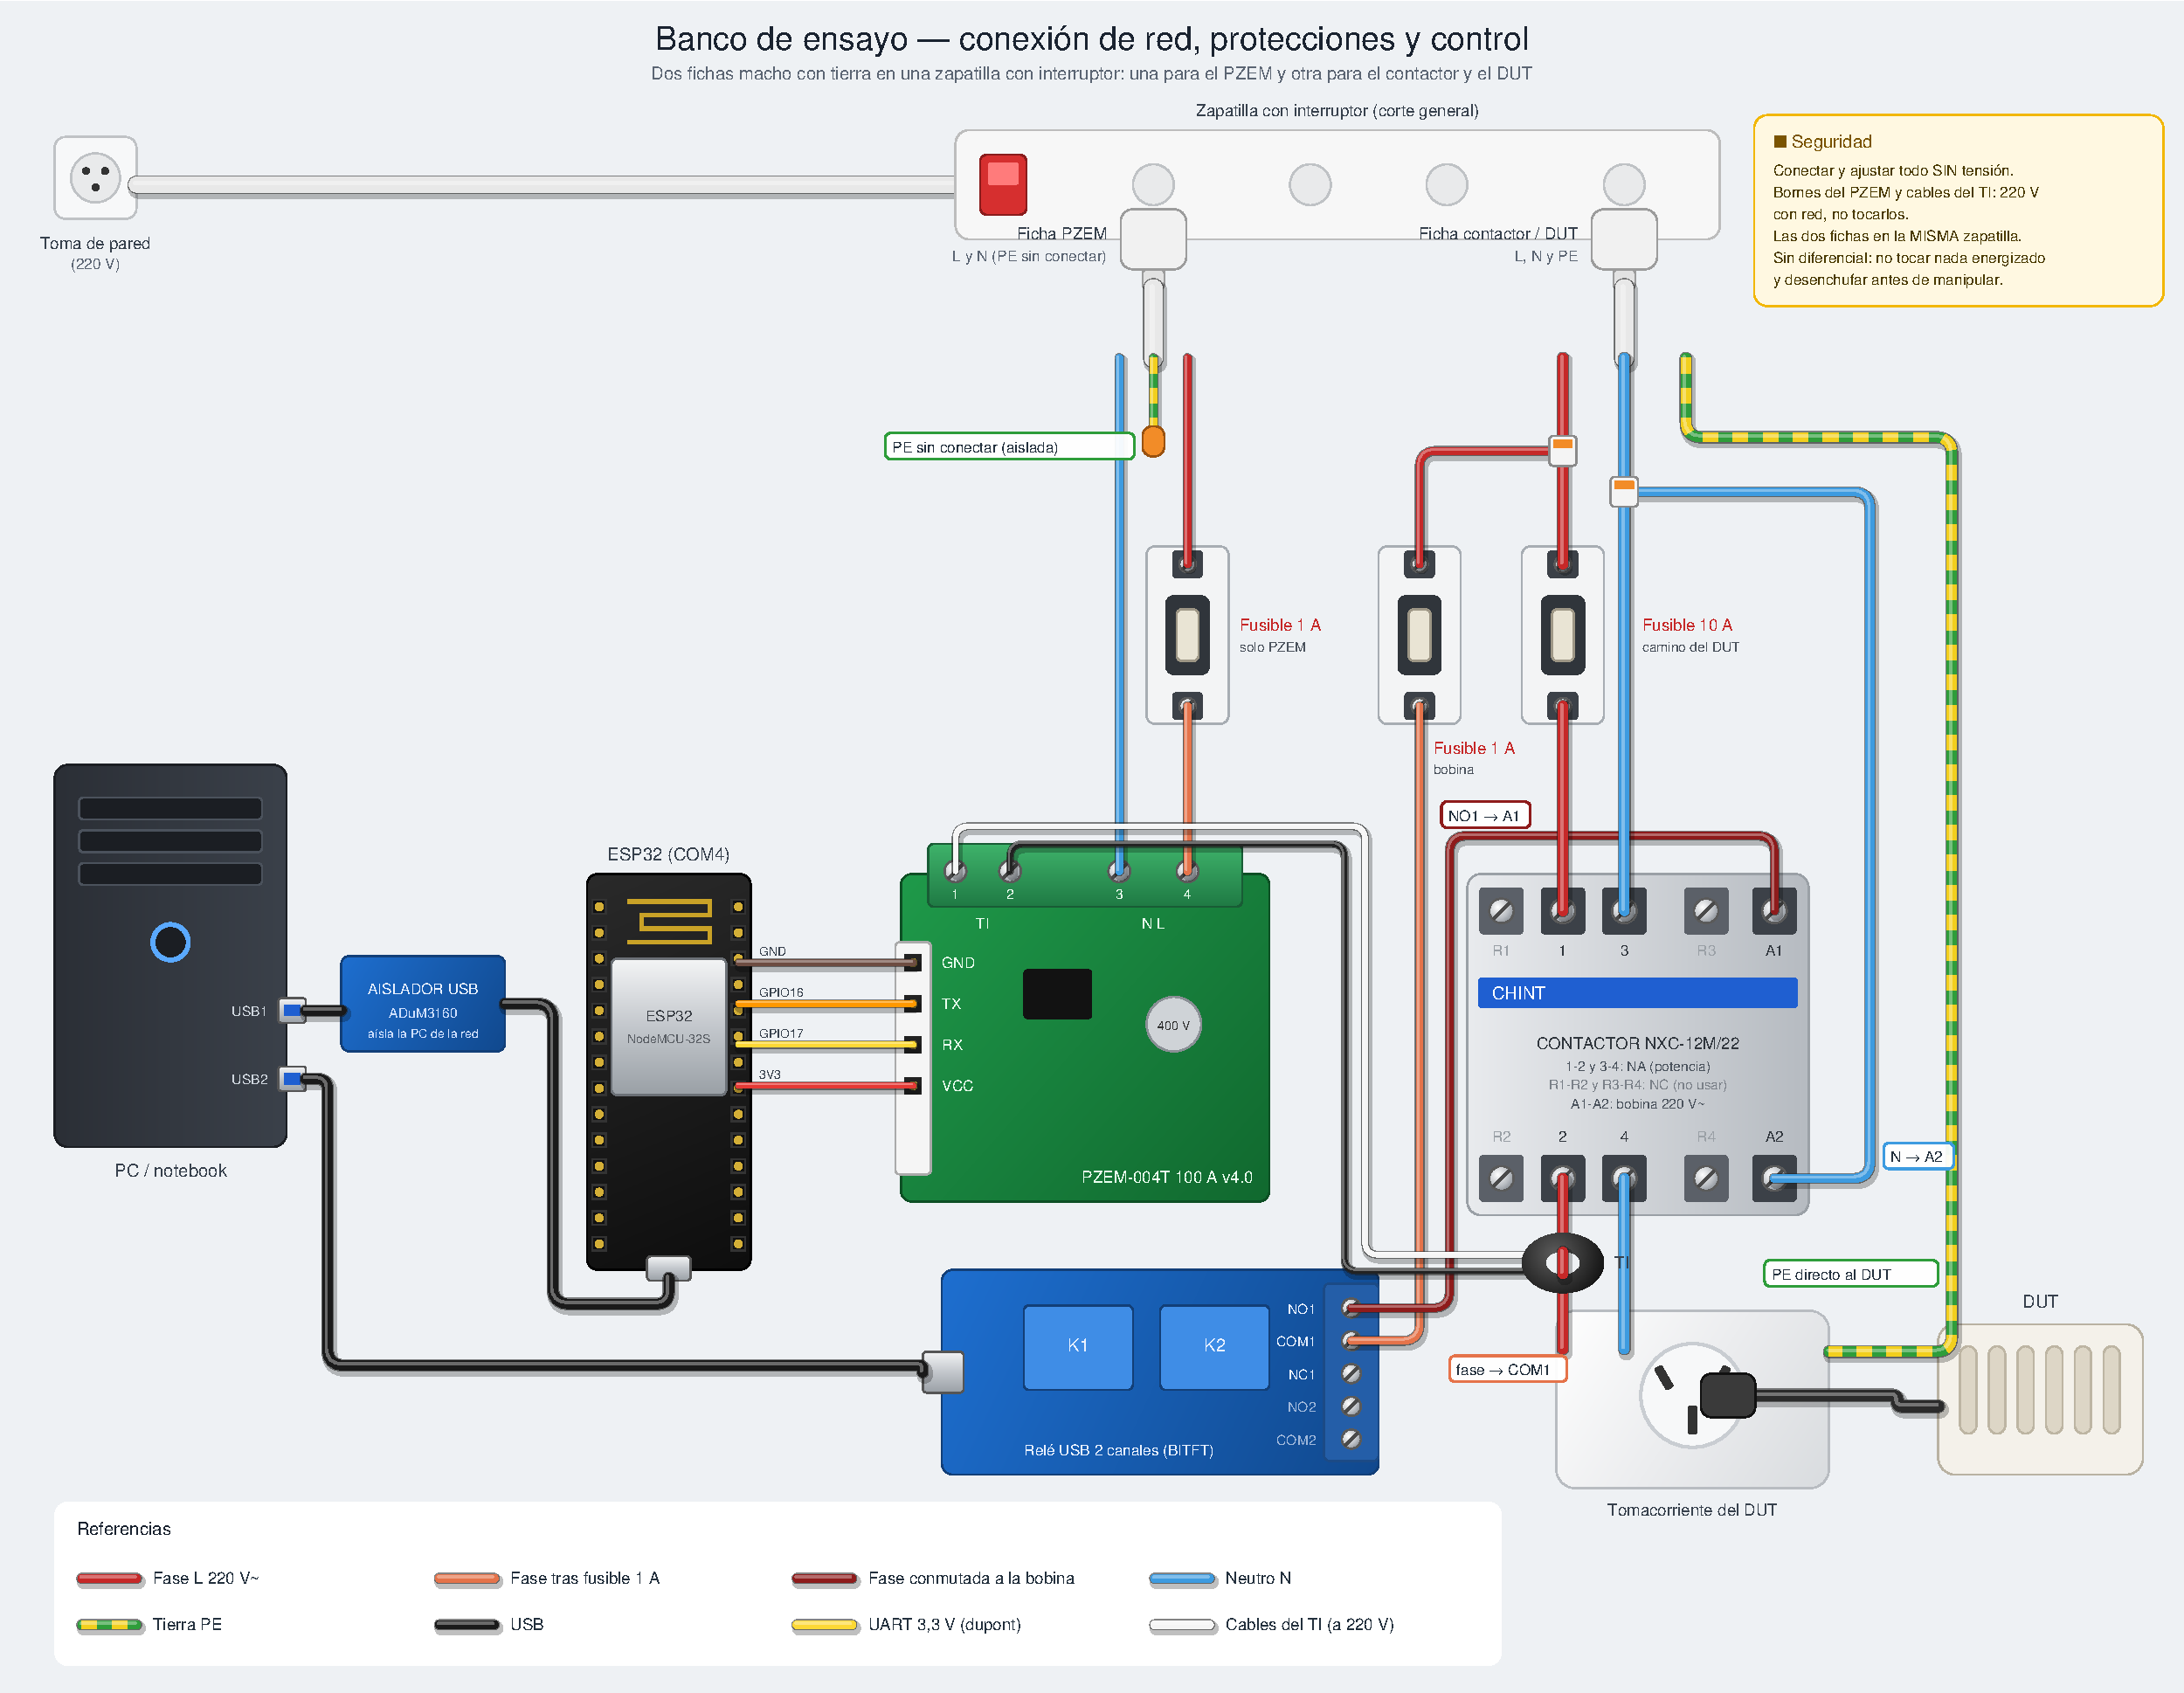
\includegraphics[width=\linewidth]{conexion_red_banco.pdf}
    \caption{Banco de pruebas: conexión de red, protecciones y control.}
    \label{fig:conexion_red}
\end{figure}

\subsubsection{Protocolo de comunicación}

\begin{itemize}
    \item \textbf{ESP32 $\leftrightarrow$ PZEM:} Modbus RTU sobre UART a
          \SI{9600}{\baud}, por el segundo puerto serie del ESP32 (GPIO16 como
          recepción y GPIO17 como transmisión). Los medidores comparten el bus y
          cada uno responde a su dirección (1, 2 y 3), que se graba en el módulo
          con un comando específico. Los medidores se alimentan desde
          \SI{3,3}{\volt} (ver Sección~\ref{subsec:dificultades}).
    \item \textbf{PC $\leftrightarrow$ ESP32:} puerto serie virtual sobre USB a
          \SI{115200}{\baud}, con un protocolo de texto de una línea por comando,
          implementado en un firmware propio: \texttt{PING}, \texttt{INFO},
          \texttt{PZEM<n>} (devuelve tensión, corriente, potencia, energía y
          factor de potencia), \texttt{SETADDR} y \texttt{RELAYON/RELAYOFF}.
    \item \textbf{PC $\leftrightarrow$ placa de relés:} protocolo USB HID,
          controlado desde Python. Después de cada orden, el software lee el
          estado de la placa para confirmar la conmutación.
\end{itemize}

% ------------------------------------------------------------
\subsection{Desarrollo del software}
\label{subsec:metodologia_sw}
% ------------------------------------------------------------

\subsubsection{Tecnologías}

El software está escrito en Python~3.11, con dependencias gestionadas mediante
\texttt{uv}. La interfaz gráfica usa PyQt5 y gráficos en vivo; la comunicación
serie, \texttt{pyserial}; el almacenamiento, SQLite; la exportación, Excel y correo
electrónico; y el acceso remoto, una API REST con FastAPI y autenticación. El
código se versiona en GitHub con integración continua que ejecuta las pruebas
automáticas, el análisis estático y una prueba en contenedor Docker.

\subsubsection{Arquitectura}

El paquete se organiza en módulos con responsabilidades separadas:
\begin{itemize}
    \item \textbf{Hardware:} cliente serie del ESP32 (detección de puerto,
          reconexión y lectura segura entre hilos), controlador de la placa de
          relés y una fachada que coordina ambos.
    \item \textbf{Motor de ensayos:} un orquestador con modos de final de línea,
          cíclico y verificación con patrones; cada ensayo se implementa como una
          clase con las etapas preparación, medición, cierre y evaluación
          (patrón \emph{Template Method}). Los veredictos son funciones puras,
          separadas de la adquisición, lo que permite probarlas en forma aislada.
    \item \textbf{Modelos y base de datos:} productos, mediciones y resultados,
          con acceso a SQLite mediante el patrón repositorio y migración
          automática del esquema.
    \item \textbf{Interfaz gráfica:} pestañas de Ensayos, Productos, Consumo,
          Configuraciones, Verificación, Exportar, Historial y Administración,
          con acceso mediante usuario y contraseña.
    \item \textbf{API y exportación:} consulta remota del historial y exportación
          a Excel o por correo.
    \item \textbf{Configuración:} umbrales, tiempos, correcciones de calibración
          y asignación de relés en un archivo de entorno, editables sin modificar
          el código.
\end{itemize}

\begin{figure}[htbp]
    \centering
    \figuraopcional{arquitectura_interfaz.png}{0.85\linewidth}
    \caption{Diagrama general de la interfaz.}
    \label{fig:arquitectura_interfaz}
\end{figure}

\subsubsection{Interfaz gráfica}

La Figura~\ref{fig:gui} muestra las pantallas principales de la aplicación: la
pestaña de Ensayos, donde el operario elige el producto y ejecuta la secuencia;
la de Consumo, con los valores en vivo y los gráficos del perfil; la de
Productos, donde se cargan los datos de placa que definen los límites; y la de
Configuraciones, con los tiempos de cada ensayo y los modos de ejecución.

\begin{figure}[htbp]
    \centering
    \begin{subfigure}[b]{0.49\linewidth}
        \centering
        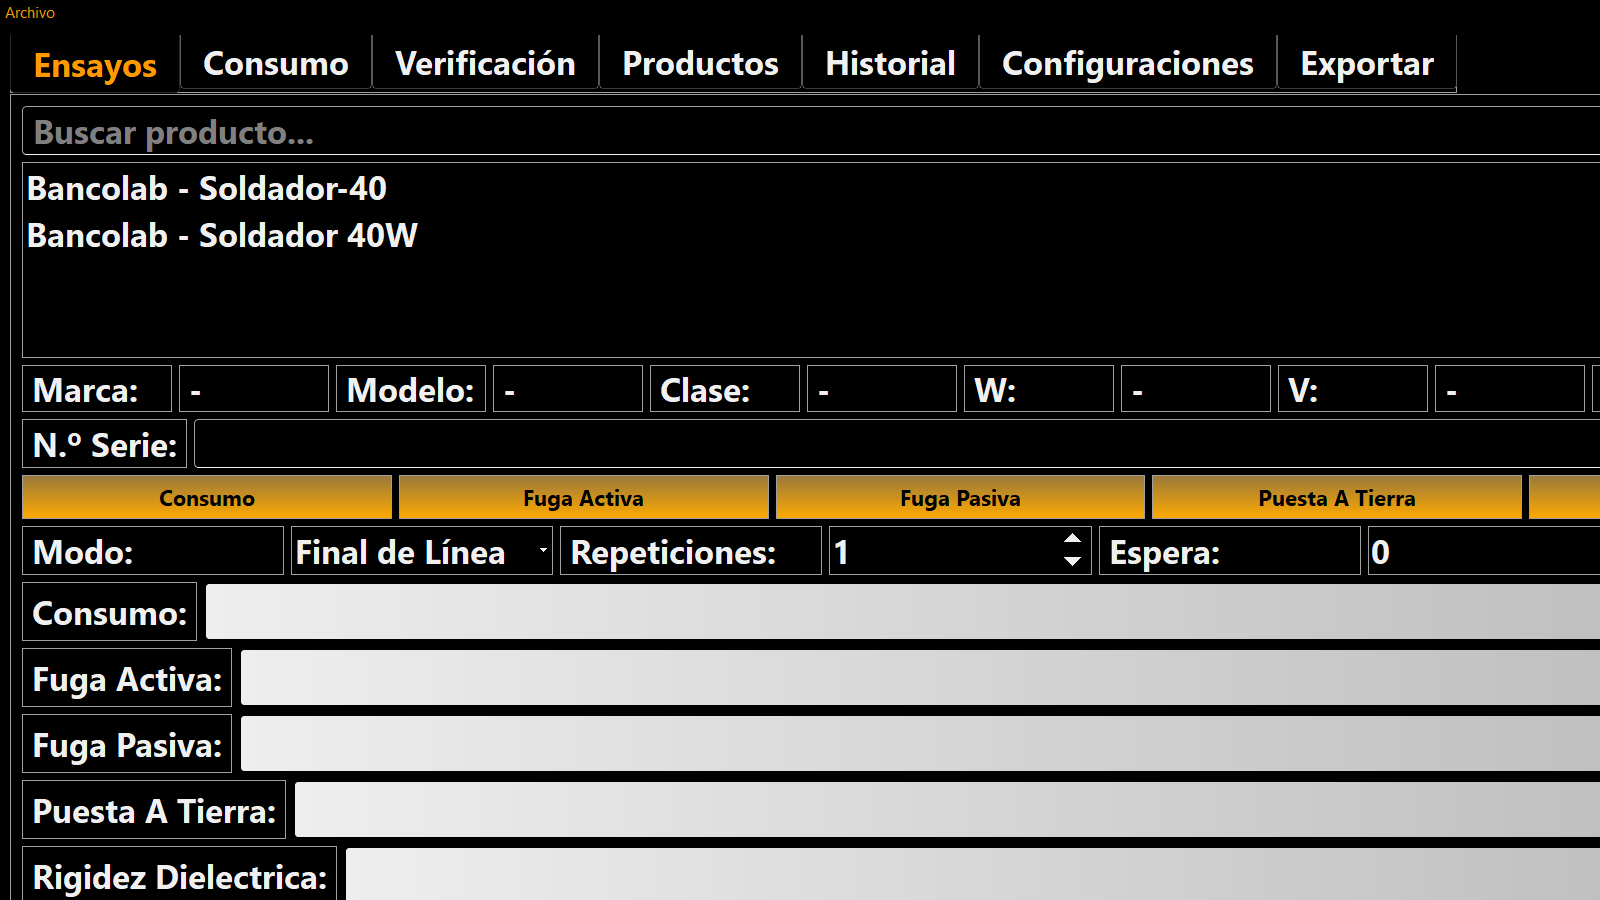
\includegraphics[width=\linewidth]{gui_ensayos.png}
        \caption{Ensayos.}
    \end{subfigure}\hfill
    \begin{subfigure}[b]{0.49\linewidth}
        \centering
        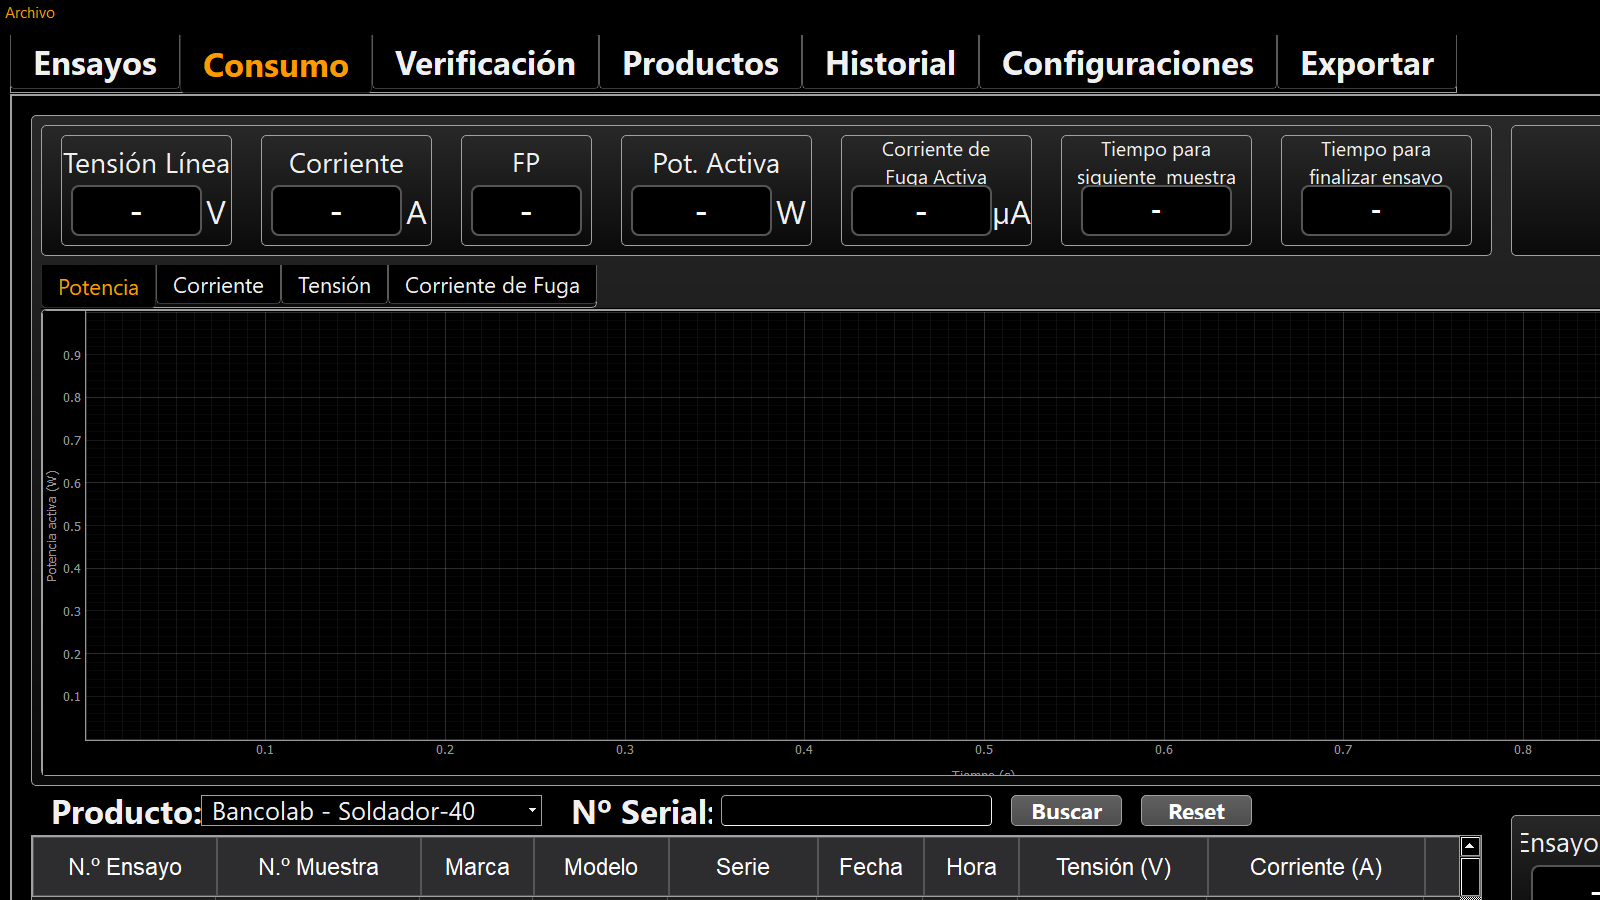
\includegraphics[width=\linewidth]{gui_consumo.png}
        \caption{Consumo.}
    \end{subfigure}\\[1em]
    \begin{subfigure}[b]{0.49\linewidth}
        \centering
        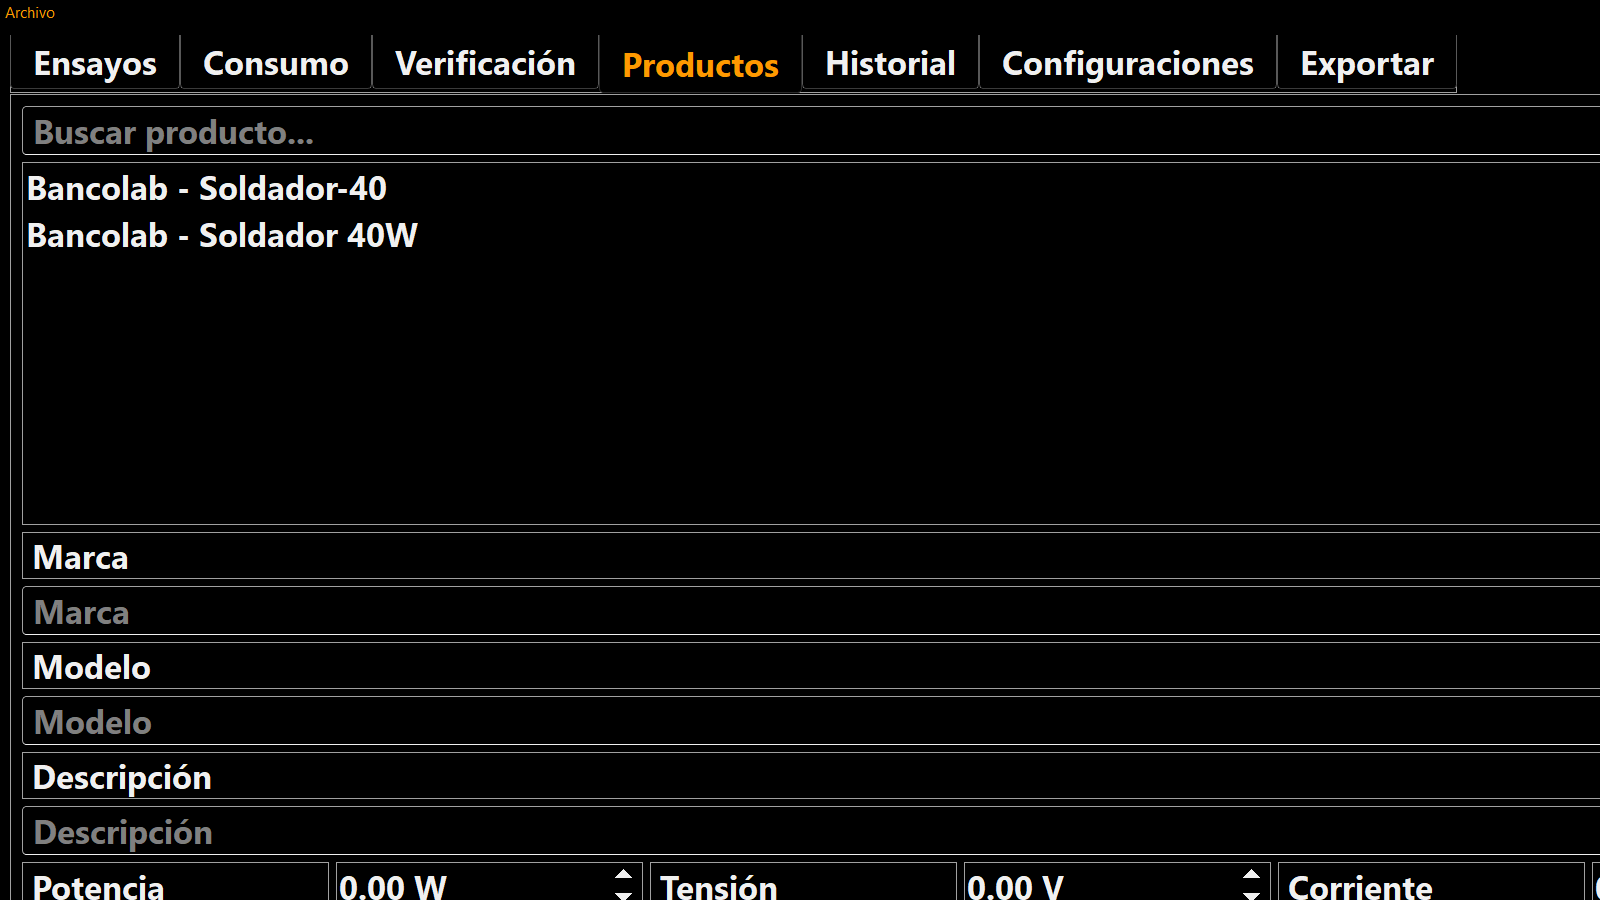
\includegraphics[width=\linewidth]{gui_productos.png}
        \caption{Productos.}
    \end{subfigure}\hfill
    \begin{subfigure}[b]{0.49\linewidth}
        \centering
        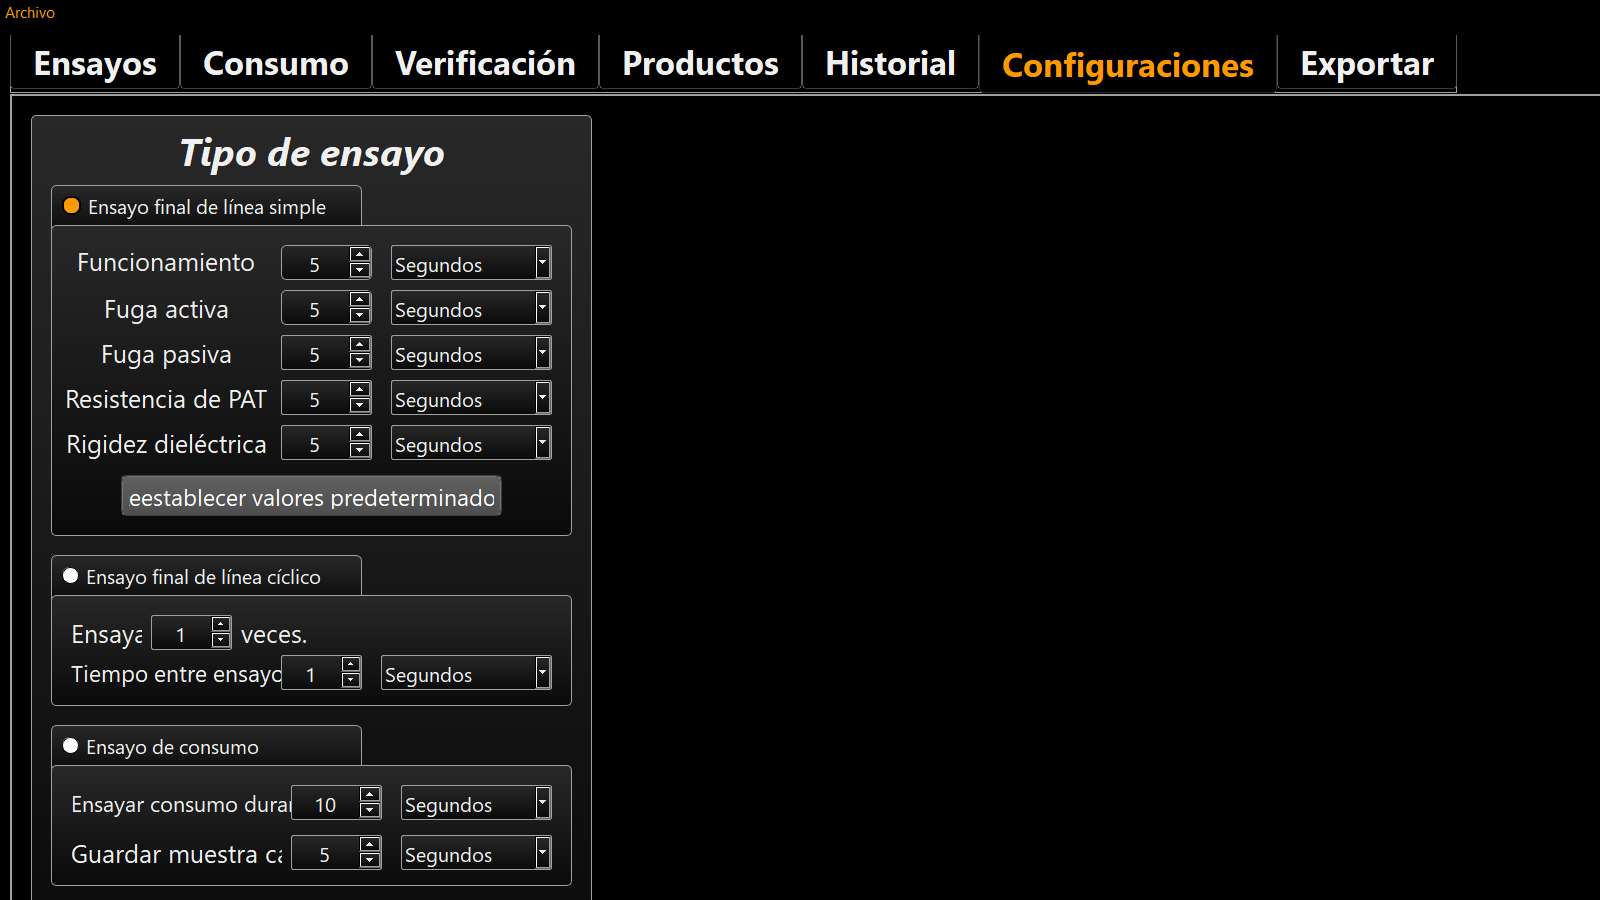
\includegraphics[width=\linewidth]{gui_configuraciones.png}
        \caption{Configuraciones.}
    \end{subfigure}
    \caption{Pantallas principales de la interfaz gráfica.}
    \label{fig:gui}
\end{figure}

% ------------------------------------------------------------
\subsection{Criterios metodológicos de los ensayos}
\label{subsec:criterios_ensayo}
% ------------------------------------------------------------

\begin{itemize}
    \item \textbf{Ensayos de rutina:} por ser un equipo de final de línea, se
          aplican los ensayos de rutina del Anexo~A (rigidez dieléctrica y
          puesta a tierra); para fuga y consumo, que el Anexo~A no contempla, se
          toman los límites de las cláusulas~13, 16 y~10.
    \item \textbf{Peor caso frente a promedio:} en rigidez dieléctrica y puesta a
          tierra el veredicto se toma sobre el peor valor del intervalo (tensión
          mínima y corriente máxima, o resistencia máxima), porque una sola lectura
          fuera de límite indica una falla de seguridad. En consumo se usa el
          promedio del intervalo, que representa la potencia en régimen.
    \item \textbf{Condiciones de validez:} si la tensión de rigidez no alcanzó el
          valor de ensayo, o si la corriente de puesta a tierra no llegó a
          \SI{10}{\ampere}, el aislamiento o la continuidad no se verificaron en
          condiciones de norma y el resultado es FALLA.
    \item \textbf{Estabilización:} en consumo se descartan las lecturas tomadas
          mientras el contactor cierra y el medidor se actualiza (dos lecturas en
          el ensayo de final de línea y \SI{3}{\second} en el perfil de consumo).
    \item \textbf{Falla segura:} en los ensayos de seguridad, una lectura fallida
          del medidor produce FALLA y nunca un aprobado; ante cualquier error, el
          software abre los relés y el contactor.
\end{itemize}

% ------------------------------------------------------------
\subsection{Procedimiento de pruebas}
\label{subsec:procedimiento_pruebas}
% ------------------------------------------------------------

\begin{itemize}
    \item \textbf{Pruebas unitarias:} cada componente del software se valida de
          forma independiente, con el hardware simulado.
    \item \textbf{Pruebas de integración:} se evalúa la interacción entre módulos,
          desde la adquisición hasta el almacenamiento y la interfaz, incluida la
          ventana principal en modo sin pantalla.
    \item \textbf{Pruebas en banco:} se opera la aplicación real con el hardware
          real sobre cargas conocidas (una resistiva y una con motor), registrando
          los resultados en una base de datos separada.
\end{itemize}

% ============================================================
%  Ensayos aplicados
% ============================================================
\section{Ensayos aplicados}
\label{sec:ensayos}

El sistema realiza los siguientes ensayos sobre aparatos de tensión nominal
mayor a \SI{150}{\volt} (\SIrange{220}{240}{\volt}). La Tabla~\ref{tab:ensayos}
resume el criterio de aprobación de cada uno; los valores completos, las
condiciones de ensayo y las tolerancias de consumo por tipo de aparato se
detallan en el Anexo~\ref{anx:valores_referencia}.

\begin{table}[htbp]
\centering
\caption{Ensayos del sistema y criterio de aprobación según IEC~60335-1}
\label{tab:ensayos}
\renewcommand{\arraystretch}{1.3}
\begin{tabularx}{\linewidth}{@{} l X l @{}}
\toprule
\textbf{Ensayo} & \textbf{Criterio de aprobación} & \textbf{Referencia} \\
\midrule
Rigidez dieléctrica
  & Corriente $\leq$ \SI{5}{\milli\ampere} con \SI{1000}{\volt} (Clase~I) o
    \SI{2500}{\volt} (Clase~II) aplicados
  & Anexo~A.2 \\
Puesta a tierra
  & $\leq$ \SI{200}{\milli\ohm} con cable fijo o $\leq$ \SI{100}{\milli\ohm} sin
    él, con corriente $\geq$ \SI{10}{\ampere}; solo Clase~I
  & Anexo~A.1 \\
Fuga activa
  & $\leq$ \SI{750}{\micro\ampere} (Clase~I portátil)
  & 13.2 \\
Fuga pasiva
  & $\leq$ \SI{750}{\micro\ampere}; \SI{1500}{\micro\ampere} solo si el aparato
    cumple una condición de duplicación
  & 16.2 \\
Consumo
  & Potencia o corriente dentro de la tolerancia según el tipo de aparato y la
    potencia nominal
  & 10.1 y 10.2 \\
\bottomrule
\end{tabularx}
\end{table}

Estos ensayos permiten detectar fallas críticas de aislamiento, de conexión a
tierra o de funcionamiento durante la etapa de producción.

% ============================================================
%  Evaluación de costos
% ============================================================
\section{Evaluación de costos}
\label{sec:costos}

El presupuesto del proyecto se fijó en \SI{1030}{USD}, distribuido por concepto
según la Tabla~\ref{tab:presupuesto}.

\begin{table}[htbp]
\centering
\caption{Presupuesto del proyecto por concepto}
\label{tab:presupuesto}
\renewcommand{\arraystretch}{1.2}
\begin{tabular}{@{} l r @{}}
\toprule
\textbf{Concepto} & \textbf{Costo (USD)} \\
\midrule
Medición de corriente de fuga activa       & 30 \\
Medición de corriente de fuga pasiva       & 30 \\
Medición de resistencia de puesta a tierra & 30 \\
Medición de rigidez dieléctrica            & 30 \\
Elementos de conexión                      & 70 \\
Elementos de medición                      & 150 \\
Elementos de seguridad                     & 60 \\
Elementos de potencia                      & 180 \\
Elementos de control                       & 50 \\
Elementos de procesamiento                 & 400 \\
Horas de trabajo                           & --- \\
\midrule
\textbf{Total}                             & \textbf{1030} \\
\bottomrule
\end{tabular}
\end{table}

La Tabla~\ref{tab:costos_detalle} presenta el costo del prototipo por componente,
a partir de un relevamiento de precios de publicaciones de Mercado Libre Argentina
realizado en noviembre de 2026, convertidos a un tipo de cambio de
\num{1570}~pesos por dólar. Para los componentes sin publicaciones comparables
(transformador de alta tensión, elementos de seguridad, conexionado y riel DIN) se
mantiene la estimación previa en dólares, indicada como ``est.''. Los precios de
las publicaciones varían entre vendedores, por lo que el total debe leerse como
un valor de referencia. Las horas de ingeniería no se incluyen, por corresponder
al esfuerzo académico del trabajo.

\begin{table}[htbp]
\centering
\caption{Costo del prototipo por componente (precios de Mercado Libre, noviembre
         de 2026; \num{1570}~ARS/USD)}
\label{tab:costos_detalle}
\renewcommand{\arraystretch}{1.2}
\small\setlength{\tabcolsep}{4pt}
\begin{tabular}{@{} l p{5.6cm} r r r @{}}
\toprule
\textbf{Categoría} & \textbf{Componente} & \textbf{Cant.} &
\textbf{Unit. (ARS)} & \textbf{Subtotal (USD)} \\
\midrule
\multirow{2}{*}{Procesamiento}
  & ESP32 NodeMCU-32S                     & 1 & \num{13500}  & 8,60  \\
  & Módulo de relés USB de 8 canales      & 1 & \num{29471}  & 18,77 \\
\midrule
\multirow{2}{*}{Medición}
  & PZEM-004T \SI{100}{\ampere} con transformador de corriente
                                          & 3 & \num{47990}  & 91,70 \\
  & Cables de medición y puntas           & --- & est.       & 10,00 \\
\midrule
\multirow{3}{*}{Potencia}
  & Minicontactor CHINT NXC-12M/22, bobina \SI{220}{\volt}
                                          & 4 & \num{30000}  & 76,43 \\
  & Transformador de rigidez dieléctrica  & 1 & est.         & 80,00 \\
  & Transformador \SI{75}{\volt\ampere} (puesta a tierra)
                                          & 1 & \num{77000}  & 49,04 \\
\midrule
\multirow{3}{*}{Seguridad}
  & Fusibles y portafusibles              & 4 & est.         & 8,00  \\
  & Pilotos indicadores                   & 4 & est.         & 6,00  \\
  & Pulsador de paro de emergencia        & 1 & est.         & 8,00  \\
\midrule
\multirow{3}{*}{Conexionado}
  & Cable \SI{1,5}{\milli\meter\squared} (\SI{10}{\meter}) & 2 & est. & 12,00 \\
  & Borneras, terminales y bridas         & --- & est.       & 8,00  \\
  & Tomacorriente y fichas                & 2 & est.         & 10,00 \\
\midrule
\multirow{2}{*}{Estructura}
  & Valija de aluminio reforzada          & 1 & \num{79909}  & 50,90 \\
  & Riel DIN y panel frontal              & 1 & est.         & 15,00 \\
\midrule
\multicolumn{4}{@{}r}{\textbf{Total}}                       & \textbf{452,44} \\
\multicolumn{4}{@{}r}{Contingencia (\SI{15}{\percent})}      & 67,87 \\
\multicolumn{4}{@{}r}{\textbf{Total con contingencia}}       & \textbf{520,31} \\
\bottomrule
\end{tabular}
\end{table}

\noindent El costo del prototipo, de unos \SI{520}{USD} con contingencia
(aproximadamente \num{817000}~pesos), se ubica en la mitad del presupuesto de
\SI{1030}{USD}. Los precios relevados son en general más altos que las
estimaciones iniciales en dólares, sobre todo en los medidores y los contactores,
pero el margen del presupuesto absorbe la diferencia.

\subsection{Comparación con soluciones comerciales}
\label{subsec:comparacion_comercial}

La Tabla~\ref{tab:comparacion_comercial} compara el prototipo con equipos
comerciales nacionales de la línea SYGlab (SYG~Group), que realizan ensayos
similares bajo IEC~60335.

\begin{table}[htbp]
\centering
\caption{Comparación entre el prototipo y equipos comerciales}
\label{tab:comparacion_comercial}
\renewcommand{\arraystretch}{1.2}
\small
\begin{tabular}{@{} l c c c @{}}
\toprule
\textbf{Característica} & \textbf{Prototipo} & \textbf{SYGlab CL12-S0} &
\textbf{SYGlab MG5} \\
\midrule
Consumo                  & Validado en banco    & \checkmark & \checkmark \\
Fuga activa y pasiva     & Implementado (software) & \checkmark & \checkmark \\
Puesta a tierra          & Implementado (software) & \checkmark & \checkmark \\
Rigidez dieléctrica      & Implementado (software) & \checkmark & \checkmark \\
Clase~I y~II             & \checkmark           & \checkmark & \checkmark \\
Canales simultáneos      & 1                    & 1          & 5 \\
Interfaz                 & PC (PyQt5)           & Pantalla integrada & Pantalla integrada \\
Registro y exportación   & SQLite, Excel, API   & QR y base de datos & QR y base de datos \\
Costo                    & $\sim$\SI{520}{USD}  & Consultar  & Consultar \\
\bottomrule
\end{tabular}
\end{table}

El prototipo cubre el mismo conjunto de ensayos que los equipos de referencia. Su
ventaja diferencial es el bajo costo de construcción, el código fuente abierto y la
posibilidad de adaptar los límites a otras normativas sin restricciones de
licencia; su principal desventaja actual es que tres de los cinco ensayos todavía
no están validados con su hardware de medición.

% ============================================================
%  Criterios de éxito y plan de validación
% ============================================================
\section{Criterios de evaluación y éxito}
\label{sec:criterios_evaluacion}

El sistema se considera exitoso si cumple con los siguientes criterios:
\begin{itemize}
    \item \textbf{Tiempo de prueba:} reducción de al menos \SI{30}{\percent} del
          tiempo de ensayo respecto de los métodos manuales, gracias a la
          secuencia automática y a la eliminación de ajustes manuales.
    \item \textbf{Automatización:} reducción de al menos \SI{80}{\percent} de la
          intervención del operario en configuración, conmutación entre ensayos y
          adquisición de datos.
    \item \textbf{Seguridad:} alarmas ante ensayos no aprobados o exposición a
          tensiones peligrosas, y comportamiento seguro ante fallas.
    \item \textbf{Escalabilidad:} adaptación a nuevos tipos de dispositivos y a
          cambios normativos sin reestructurar el sistema.
    \item \textbf{Cumplimiento normativo:} ensayos realizados conforme a la
          IEC~60335 y mediciones evaluadas contra sus límites, con trazabilidad.
    \item \textbf{Cronograma:} respeto de las fases y plazos planificados
          (Anexo~\ref{anx:cronograma}), con una tolerancia máxima de diez días.
    \item \textbf{Presupuesto:} costo de desarrollo dentro de \SI{1030}{USD},
          con un margen razonable solo ante contingencias justificadas.
\end{itemize}

\section{Plan de validación}
\label{sec:plan_validacion}

La validación se plantea en tres niveles complementarios: hardware, software y
sistema integrado.

\subsection{Validación del hardware}
\begin{itemize}
    \item \textbf{Verificación funcional:} cada módulo (alimentación, protección,
          medición y desconexión) se evalúa por separado frente a sus
          especificaciones.
    \item \textbf{Pruebas de seguridad:} aislamiento, funcionamiento de las
          protecciones y activación de alarmas ante fallas.
    \item \textbf{Calibración:} contraste con instrumentos patrón certificados,
          cuya incertidumbre sea al menos diez veces menor que la del
          dispositivo.
\end{itemize}

\subsection{Validación del software}
\begin{itemize}
    \item \textbf{Pruebas unitarias:} veredictos, ensayos con hardware simulado,
          relés, base de datos y pestañas de la interfaz.
    \item \textbf{Pruebas de integración:} comunicación entre módulos y con el
          hardware, y correcta transferencia y almacenamiento de datos.
    \item \textbf{Usabilidad y seguridad:} configuración y ejecución intuitivas,
          con mensajes claros de error o advertencia.
\end{itemize}

\subsection{Validación del sistema frente a la norma IEC~60335}
\begin{itemize}
    \item \textbf{Ensayos comparativos:} mediciones con el prototipo y con un
          instrumento calibrado comercial, para verificar la concordancia dentro
          del margen normativo.
    \item \textbf{Verificación con patrones:} el sistema incluye un modo en el que
          se ensayan dos patrones conocidos; el primero debe aprobar y el segundo
          fallar en fuga, puesta a tierra y rigidez, y cada medición debe quedar
          dentro de \SI{\pm 10}{\percent} del valor del patrón.
    \item \textbf{Intercomparación:} cuando sea posible, contraste con resultados
          emitidos por un laboratorio acreditado.
    \item \textbf{Criterio de aceptación:} el sistema es válido si emite el
          veredicto correcto frente a los límites de la norma
          (Anexo~\ref{anx:valores_referencia}) con trazabilidad demostrable.
\end{itemize}

% ============================================================
%  Resultados y análisis
%  Solo resultados y su lectura; el desarrollo estadístico y de
%  incertidumbre está en el Anexo C.
% ============================================================
\section{Resultados y análisis}
\label{sec:resultados}

Los resultados provienen de dos fuentes
(Sección~\ref{subsubsec:equipo_syglab}): los registros del equipo completo de
referencia provisto por SYGlab, que ejecutó los ensayos de seguridad con la
versión inicial del software (Sección~\ref{subsec:resultados_syglab}), y las pruebas de la versión
final en el prototipo propio, armado con los componentes descritos en la
Sección~\ref{subsec:metodologia_hw} (Figura~\ref{fig:conexion_red}) y operado
con la aplicación y el hardware reales.
En el prototipo se usaron dos cargas: un soldador de
\SI{40}{\watt} declarados (carga resistiva) y un ventilador (carga con motor). La
evidencia ---fotografías, base de datos, exportación y scripts de prueba--- se
lista en el Anexo~\ref{anx:evidencia}.

Al momento de las pruebas no se había realizado el contraste con el instrumento
patrón previsto (Sección~\ref{subsec:metodologia_hw}), por lo que los
resultados verifican el funcionamiento del sistema y la corrección de sus
veredictos, pero \textbf{no constituyen una validación metrológica}.

% ------------------------------------------------------------
\subsection{Ensayo de consumo}
\label{subsec:resultados_consumo}
% ------------------------------------------------------------

La Tabla~\ref{tab:resultados_consumo} resume las mediciones con carga. La tensión
de red medida varió entre \SIlist{226;231}{\volt} a lo largo de los días de
prueba.

\begin{table}[htbp]
\centering
\caption{Mediciones de consumo en el banco de pruebas}
\label{tab:resultados_consumo}
\renewcommand{\arraystretch}{1.25}
\small\setlength{\tabcolsep}{4pt}
\begin{tabular}{@{} l p{3.6cm} c c c c @{}}
\toprule
\textbf{Carga} & \textbf{Prueba} & \textbf{$V$ [\si{\volt}]} &
\textbf{$I$ [\si{\ampere}]} & \textbf{$P$ [\si{\watt}]} & \textbf{FP} \\
\midrule
Ventilador & Lectura directa
  & 228,7--228,9 & 0,236--0,242 & 52,1--53,4 & 0,96--0,97 \\
Soldador   & Lectura directa
  & 230,1--230,2 & 0,163--0,164 & 37,5--37,7 & 1,00 \\
Soldador   & Final de línea, 4 ensayos
  & 227,7--228,0 & 0,161--0,162 & 36,6--36,8 & 0,99--1,00 \\
Soldador   & Perfil de consumo, 8 muestras
  & 226,2--227,3 & 0,160--0,161 & 36,1--36,4 & 1,00 \\
\bottomrule
\end{tabular}
\end{table}

Para el soldador, configurado como aparato de calefacción de \SI{40}{\watt}, la
tolerancia aplicable es de \SI{\pm 10}{\percent} (\SIrange{36}{44}{\watt}). La
Tabla~\ref{tab:resultados_veredicto} resume el resultado del ensayo de final de
línea.

\begin{table}[htbp]
\centering
\caption{Veredicto del ensayo de consumo del soldador}
\label{tab:resultados_veredicto}
\renewcommand{\arraystretch}{1.25}
\begin{tabular}{@{} l r @{}}
\toprule
\textbf{Parámetro} & \textbf{Valor} \\
\midrule
Potencia nominal declarada        & \SI{40}{\watt} \\
Intervalo admisible (calefacción, \SIrange{25}{200}{\watt}) & \SIrange{36}{44}{\watt} \\
Potencia media medida ($n = 4$)   & \SI{36,70}{\watt} \\
Desviación respecto del nominal   & \SI{-8,3}{\percent} \\
Coeficiente de variación          & \SI{0,22}{\percent} \\
Incertidumbre expandida ($k = 2$) & \SI{0,23}{\watt} \\
\midrule
\textbf{Veredicto del sistema}    & \textbf{OK} \\
\bottomrule
\end{tabular}
\end{table}

\paragraph{Análisis.}
\begin{itemize}
    \item La \textbf{repetibilidad} es muy buena: los cuatro ensayos de final de
          línea difieren en \SI{0,2}{\watt} y el coeficiente de variación es del
          \SI{0,22}{\percent}, del mismo orden que la resolución del medidor.
    \item La \textbf{incertidumbre} estimada (\SI{0,23}{\watt}) es pequeña frente
          al ancho de la banda de tolerancia (\SI{\pm 4}{\watt}), por lo que la
          dispersión del sistema no compromete el veredicto. El desarrollo del
          cálculo está en el Anexo~\ref{anx:estadistica}.
    \item El resultado queda \textbf{cerca del límite inferior} (\SI{36}{\watt}).
          La cláusula~10.1 pide medir a la tensión nominal y el banco mide a la
          tensión de red disponible, sin regularla. El soldador está marcado para
          \SI{230}{\volt}; como en una carga resistiva la potencia varía con el
          cuadrado de la tensión, su consumo a la tensión nominal se estima en
          \SI{37,4}{\watt} (\SI{-6,6}{\percent}), con lo que el veredicto se
          mantiene. En un aparato más cercano al límite, en cambio, la tensión de
          ensayo podría cambiar el veredicto; el Anexo~\ref{anx:estadistica}
          desarrolla este efecto.
    \item Las lecturas del perfil (\SI{36,2}{\watt} en promedio) son
          \SI{0,5}{\watt} menores que las de final de línea, coherente con la
          menor tensión de red en ese momento (\SI{227}{\volt} frente a
          \SI{228}{\volt}).
\end{itemize}

% ------------------------------------------------------------
\subsection{Prueba de punta a punta}
\label{subsec:resultados_e2e}
% ------------------------------------------------------------

La prueba de punta a punta recorrió la aplicación completa sobre el
banco: detección del hardware, alta de productos, ensayos de final de línea y
cíclico, parada de emergencia, cierre de la ventana durante un ensayo, historial,
exportación y API. Encontró seis defectos, que se corrigieron y se volvieron a
verificar en el banco (Tabla~\ref{tab:resultados_e2e}).

\begin{table}[htbp]
\centering
\caption{Defectos encontrados en la prueba de punta a punta y verificación de la
         corrección en el banco}
\label{tab:resultados_e2e}
\renewcommand{\arraystretch}{1.25}
\small
\begin{tabularx}{\linewidth}{@{} l X X @{}}
\toprule
\textbf{Área} & \textbf{Antes} & \textbf{Después de la corrección} \\
\midrule
Consumo (soldador)
  & \SIlist{27,2;33,2;31,6;32,6}{\watt}: FALLA
  & \SIlist{36,8;36,7;36,7;36,6}{\watt}: OK \\
Modo cíclico
  & La interfaz se liberaba tras el primer ciclo
  & Bloqueada hasta el tercer ciclo (\SI{22,1}{\second}) \\
Error durante un ensayo
  & Interfaz bloqueada, sin aviso
  & Aviso visible, interfaz libre en \SI{0,5}{\second}, relés abiertos \\
Fuga sin medidor
  & NO EJECUTADO
  & FALLA (lectura fallida = FALLA) \\
Historial
  & Columnas de corriente y potencia vacías
  & Completas, con la resolución del medidor \\
Cierre durante un ensayo
  & El ensayo seguía unos \SI{4}{\second}
  & Se detiene en \SI{0,4}{\second}, relés abiertos \\
\bottomrule
\end{tabularx}
\end{table}

El defecto más relevante fue la \textbf{subestimación del consumo en un
\SI{27}{\percent}}: el promedio incluía lecturas tomadas mientras el contactor
cerraba (\SI{0}{\watt}, luego \SI{26}{\watt} y recién después \SI{37}{\watt}), y
un aparato en buen estado resultaba rechazado. Se corrigió descartando las
lecturas de estabilización (Sección~\ref{subsec:criterios_ensayo}). Además, la
parada de emergencia cortó el ensayo en \SI{0,6}{\second} con los relés abiertos,
y la exportación generó un archivo Excel con las hojas de historial, consumo y
verificación.

% ------------------------------------------------------------
\subsection{Ensayos en el equipo completo de SYGlab}
\label{subsec:resultados_syglab}
% ------------------------------------------------------------

La base de datos de la versión inicial del software, instalada en el equipo de
SYGlab, registra \textbf{86 verificaciones con patrones} realizadas en 18
jornadas entre 2023 y 2025. En cada verificación el equipo ensaya dos patrones
conocidos ---uno que debe aprobar y otro que debe fallar--- en corte de neutro,
puesta a tierra y tensión resistida, y registra si obtuvo el resultado esperado
(OK) o no (ERROR). La Tabla~\ref{tab:verificaciones_fdl} resume los resultados;
la base registra además tres ensayos de consumo de un producto Indelplas IV~20.

\begin{table}[htbp]
\centering
\caption{Verificaciones con patrones del equipo completo de SYGlab (versión inicial
         del software, 2023 a 2025)}
\label{tab:verificaciones_fdl}
\renewcommand{\arraystretch}{1.25}
\small
\begin{tabular}{@{} l c c c c c @{}}
\toprule
& \multicolumn{2}{c}{\textbf{Patrón que debe aprobar}}
& \multicolumn{3}{c}{\textbf{Patrón que debe fallar}} \\
\cmidrule(lr){2-3}\cmidrule(l){4-6}
\textbf{Ensayo} & \textbf{OK} & \textbf{ERROR} & \textbf{OK} & \textbf{ERROR} &
\textbf{No ensayado} \\
\midrule
Corte de neutro    & 86 & 0  & 76 & 0 & 10 \\
Puesta a tierra    & 42 & 44 & 69 & 7 & 10 \\
Tensión resistida  & 84 & 2  & 69 & 7 & 10 \\
\bottomrule
\end{tabular}
\end{table}

\paragraph{Análisis.}
\begin{itemize}
    \item El corte de neutro y la tensión resistida se comportaron de forma
          consistente: el patrón que debe aprobar dio el resultado esperado en
          el \SI{100}{\percent} y el \SI{98}{\percent} de las verificaciones.
    \item La \textbf{puesta a tierra} fue la medición más sensible: el patrón que
          debe aprobar resultó en ERROR en 44 de las 86 verificaciones. Coincide
          con que el sistema tenía configurada una corrección de calibración de
          puesta a tierra, y con lo observado en el diseño de este trabajo: la
          medición de resistencias de pocos miliohmios depende de la corriente de
          ensayo (al menos \SI{10}{\ampere}), de la resistencia de contacto y del
          método de medición (Anexo~\ref{anx:valores_referencia}). Esto motivó
          exigir en la versión final que la corriente alcance el mínimo de la
          norma para dar por válido el ensayo.
    \item Solo 39 de las 86 verificaciones resultaron completamente correctas en
          los seis controles, lo que muestra el valor de verificar el equipo con
          patrones antes de cada jornada, función que la versión final conserva.
\end{itemize}

% ------------------------------------------------------------
\subsection{Ensayos de seguridad con la versión final}
\label{subsec:resultados_seguridad}
% ------------------------------------------------------------

En la versión final, los ensayos de fuga, puesta a tierra y rigidez dieléctrica
están implementados con los límites de la norma y verificados con hardware
simulado. Su ejecución con hardware real corresponde a la versión inicial en el
equipo de SYGlab (Sección~\ref{subsec:resultados_syglab}): el prototipo propio no
incluye su hardware de medición, y no hay registros de la versión final en
aquel equipo (Tabla~\ref{tab:estado_ensayos}). En el prototipo se comprobó que, sin ese
hardware, el sistema responde de forma segura: informa FALLA y deja los relés
abiertos.

\begin{table}[htbp]
\centering
\caption{Estado de cada ensayo al cierre del trabajo}
\label{tab:estado_ensayos}
\renewcommand{\arraystretch}{1.25}
\small
\begin{tabularx}{\linewidth}{@{} l l X @{}}
\toprule
\textbf{Ensayo} & \textbf{Estado} & \textbf{Falta para validarlo en banco} \\
\midrule
Consumo (final de línea, perfil, cíclico) & Validado en banco & Contraste con patrón \\
Fuga activa y pasiva & Software verificado
  & PZEM-004T de \SI{10}{\ampere} y red de medición IEC~60990 \\
Puesta a tierra & Software verificado
  & PZEM3, transformador de \SI{2,2}{\volt} y verificar $\geq$ \SI{10}{\ampere} \\
Rigidez dieléctrica & Software verificado
  & Transformador de alta tensión y medición de \SI{5}{\milli\ampere} \\
Verificación con patrones & Software verificado & Hardware de los tres ensayos anteriores \\
\bottomrule
\end{tabularx}
\end{table}

% ------------------------------------------------------------
\subsection{Calidad del software}
\label{subsec:resultados_software}
% ------------------------------------------------------------

Las pruebas automáticas pasaron de 63 a 158 a lo largo del período y cubren los
veredictos de la norma, las tolerancias de consumo, los ensayos con hardware
simulado, los relés (incluida la reconexión), las correcciones de calibración, las
credenciales y todas las pestañas de la interfaz. La integración continua, que no
ejecutaba las pruebas desde el primer commit por un error de configuración, quedó
en verde en sus tres etapas: pruebas, análisis estático y prueba en Docker.

% ------------------------------------------------------------
\subsection{Tiempo de ensayo e intervención del operario}
\label{subsec:resultados_tiempos}
% ------------------------------------------------------------

Como no se realizó una medición comparativa con un operario ensayando con
instrumentos convencionales, la Tabla~\ref{tab:tiempos} presenta una
\textbf{estimación} por aparato. Para el método manual se considera que cada
ensayo exige conectar el instrumento, configurarlo, ejecutar y anotar el
resultado; para el sistema, la duración configurada de cada ensayo
(\SI{5}{\second}) más la conmutación, coherente con lo observado en el banco
(tres ciclos de consumo en \SI{22,1}{\second}).

\begin{table}[htbp]
\centering
\caption{Estimación del tiempo y de las intervenciones del operario por aparato}
\label{tab:tiempos}
\renewcommand{\arraystretch}{1.25}
\small
\begin{tabularx}{\linewidth}{@{} X r r @{}}
\toprule
\textbf{Etapa} & \textbf{Manual} & \textbf{Sistema} \\
\midrule
Conexión del aparato y configuración          & \SI{75}{\second} & \SI{40}{\second} \\
Consumo                                       & \SI{60}{\second} & \multirow{5}{*}{\SI{30}{\second}} \\
Fuga activa                                   & \SI{45}{\second} & \\
Fuga pasiva                                   & \SI{45}{\second} & \\
Puesta a tierra                               & \SI{45}{\second} & \\
Rigidez dieléctrica                           & \SI{60}{\second} & \\
Registro de resultados                        & \SI{60}{\second} & automático \\
\midrule
\textbf{Tiempo total por aparato}             & \textbf{\SI{6,5}{\minute}}
                                              & \textbf{\SI{70}{\second}} \\
\textbf{Intervenciones del operario}          & \textbf{21} & \textbf{4} \\
\bottomrule
\end{tabularx}
\end{table}

Con estas estimaciones, el sistema reduce el tiempo de ensayo en torno al
\SI{80}{\percent} y las intervenciones del operario de 21 (conectar, configurar,
iniciar y anotar en cada uno de los cinco ensayos, y desconectar) a 4 (conectar,
elegir el producto, iniciar y desconectar), es decir, un \SI{81}{\percent}.
Ambos valores deben confirmarse con mediciones cuando estén operativos los cinco
ensayos.

% ------------------------------------------------------------
\subsection{Evaluación de los criterios de éxito}
\label{subsec:resultados_criterios}
% ------------------------------------------------------------

\begin{table}[htbp]
\centering
\caption{Evaluación de los criterios de éxito}
\label{tab:criterios_exito}
\renewcommand{\arraystretch}{1.25}
\small
\begin{tabularx}{\linewidth}{@{} l l X @{}}
\toprule
\textbf{Criterio} & \textbf{Meta} & \textbf{Resultado} \\
\midrule
Tiempo de prueba & $\geq$ \SI{30}{\percent} menos
  & Cumplido según la estimación: alrededor de \SI{80}{\percent} menos
    (Tabla~\ref{tab:tiempos}); a confirmar con mediciones \\
Intervención del operario & $\geq$ \SI{80}{\percent} menos
  & Cumplido según la estimación: de 21 a 4 intervenciones
    (\SI{81}{\percent} menos); a confirmar con mediciones \\
Seguridad & Alarmas y falla segura
  & Cumplido en el banco: relés abiertos ante error, parada y cierre;
    lectura fallida = FALLA \\
Escalabilidad & Adaptable a productos y normas
  & Cumplido: límites por atributos del producto y umbrales configurables \\
Cumplimiento normativo & Límites IEC~60335
  & Límites alineados con la norma; consumo validado; trazabilidad metrológica
    pendiente de patrón \\
Cronograma & Tolerancia de 10 días
  & Cumplido: el hardware se demoró unos días por los envíos de componentes,
    dentro de la tolerancia, y el software se adelantó unas dos semanas
    (Anexo~\ref{anx:cronograma}) \\
Presupuesto & $\leq$ \SI{1030}{USD}
  & Cumplido: unos \SI{520}{USD} con contingencia
    (Tabla~\ref{tab:costos_detalle}) \\
\bottomrule
\end{tabularx}
\end{table}

% ============================================================
%  Conclusiones
% ============================================================
\section{Conclusiones}
\label{sec:conclusiones}

El objetivo del trabajo fue diseñar y construir un sistema semiautomatizado,
formado por un dispositivo y una interfaz de software, capaz de ejecutar en final
de línea los ensayos de seguridad eléctrica de la norma IEC~60335 con precisión,
repetibilidad y trazabilidad, y con menor intervención y riesgo para el operario.
Al cierre del trabajo, ese objetivo se cumple en forma completa para el ensayo de
consumo y en forma parcial para los ensayos de seguridad, cuya lógica está
terminada pero cuyo hardware de medición está pendiente.

\subsection{Logros respecto del objetivo y el alcance}

\begin{itemize}
    \item Se construyó un \textbf{sistema integrado y funcional}: el software
          detecta el hardware, comanda los relés y el contactor, lee los
          medidores, emite el veredicto, registra cada ensayo y lo exporta. El
          ensayo de consumo quedó validado de punta a punta sobre cargas reales,
          en sus modos de final de línea, perfil y cíclico, con una repetibilidad
          del \SI{0,22}{\percent}.
    \item Se \textbf{esquematizó el equipo completo de SYGlab}, que sirvió de
          referencia para la arquitectura y para los esquemas de conexión de los
          ensayos de seguridad. Sus registros (86 verificaciones con patrones
          entre 2023 y 2025) mostraron que la puesta a tierra era la medición más
          delicada, lo que orientó los criterios de validez del software nuevo.
    \item Los \textbf{criterios de aprobación quedaron alineados con la norma}.
          La revisión de la IEC~60335-1 mostró que los límites de partida no la
          reflejaban: la rigidez dieléctrica se evaluaba solo por tensión, la fuga
          pasiva tenía un límite fijo de \SI{1500}{\micro\ampere}, la puesta a
          tierra usaba un valor único y el consumo porcentajes fijos. Se
          adoptaron los ensayos de rutina del Anexo~A y las tablas de tolerancia
          de la cláusula~10, y los límites pasaron a depender de los atributos de
          cada producto.
    \item El \textbf{software pasó de un esqueleto a una aplicación completa}: la
          interfaz inicial tenía mayormente botones sin lógica y hoy integra las
          ocho pestañas previstas, con 158 pruebas automáticas y una integración
          continua que efectivamente verifica cada cambio.
    \item Se escribió el \textbf{firmware del microcontrolador}, que no existía:
          el módulo venía con un firmware de fábrica que no atendía a los
          medidores.
    \item Se priorizó la \textbf{seguridad del operario}: el sistema nunca emite
          un aprobado ante una lectura fallida, abre los relés ante cualquier
          error, y la parada de emergencia y el cierre de la aplicación detienen el
          ensayo en menos de un segundo.
\end{itemize}

\subsection{Dificultades encontradas y cómo se resolvieron}
\label{subsec:dificultades}

\paragraph{Límites normativos mal interpretados.}
Los valores de la tabla de cotas de la formulación inicial (\SI{125}{\milli\ohm}
para puesta a tierra, \SI{50}{\milli\ampere} para rigidez dieléctrica o
\SI{\pm 10}{\percent} fijo para consumo) no coincidían con la norma. En
particular, la corriente de la fuente de alta tensión se había tomado como límite
de aprobación, cuando el criterio de la norma es de \SI{5}{\milli\ampere}. Se resolvió con una lectura detallada de la
norma, distinguiendo los ensayos de tipo de los de rutina, y con pruebas
automáticas que fijan cada límite.

\paragraph{Puesta en marcha del microcontrolador.}
El ESP32 no era reconocido (el cable USB era solo de carga, y luego faltaba el
controlador del conversor CP2102), y una vez conectado al medidor entraba en un
bucle de reinicio. La causa era doble: el medidor estaba en los pines del puerto
USB y, alimentado con \SI{5}{\volt}, su salida de datos imponía \SI{5}{\volt} en
un pin del ESP32 y le impedía arrancar. Se resolvió moviendo el medidor al
segundo puerto serie y alimentándolo desde \SI{3,3}{\volt}. Los bornes de potencia
del medidor, sin serigrafía, se identificaron midiendo con multímetro.

\paragraph{Interferencia electromagnética en el control de los relés.}
La placa de relés USB se desconectaba de la PC al abrir el contactor con una carga
con motor; con la carga resistiva no ocurría. La placa implementa el USB por
software en un microcontrolador pequeño, muy sensible a las perturbaciones que
genera la apertura de una carga inductiva. Se mitigó en dos frentes: el software
pasó a tolerar la desconexión (reintenta, confirma que los relés quedaron abiertos
o pide cortar la red) y se aprovechó que, al reiniciarse, la placa deja los relés
abiertos, lo que hace que la falla sea segura; además, se agregó un varistor en la
bobina del contactor, que redujo el problema sin eliminarlo. Fue la principal
lección de diseño del trabajo: los supresores en las bobinas, la aislación
galvánica del USB y la elección de controladores con USB por hardware deben
considerarse desde el inicio.

\paragraph{Subestimación del consumo.}
La prueba de punta a punta reveló que el consumo se subestimaba en un
\SI{27}{\percent} porque el promedio incluía las lecturas del transitorio de cierre
del contactor, lo que hacía fallar a un aparato sano. Se corrigió descartando las
lecturas de estabilización y se verificó en el banco. Esta dificultad muestra el
valor de probar con el hardware real: las pruebas con hardware simulado no podían
detectarla.

\paragraph{Calidad del proceso de software.}
La integración continua estaba mal configurada desde el primer commit y nunca
había ejecutado las pruebas ni el análisis estático; además, las correcciones de
calibración configuradas nunca se aplicaban y la API tenía credenciales de fábrica
en texto plano. Se corrigieron los tres puntos: la integración continua quedó en
verde, las correcciones se aplican a todas las lecturas y las contraseñas se
guardan con hash, rechazando las de fábrica.

\paragraph{Plazos de los componentes.}
Las demoras en los envíos de algunos componentes retrasaron unos días la
construcción del prototipo. El impacto se compensó con el adelanto del software:
el uso de herramientas de programación asistida por inteligencia artificial
permitió completar la implementación y las pruebas alrededor de dos semanas antes
de lo previsto, y ese tiempo se reinvirtió en la integración y en las pruebas en
el banco (Anexo~\ref{anx:cumplimiento_cronograma}).

\subsection{Limitaciones}

\begin{itemize}
    \item Los ensayos de fuga, puesta a tierra y rigidez dieléctrica del software
          nuevo no se ejecutaron con hardware real: el prototipo propio no incluye
          su hardware de medición, y en el equipo de SYGlab solo hay registros del
          sistema anterior.
    \item No se contó con un instrumento patrón: los resultados no constituyen
          una validación metrológica y las correcciones de calibración no están
          ajustadas.
    \item El banco mide a la tensión de red disponible y no a la tensión nominal
          del aparato, lo que afecta el veredicto de aparatos cercanos al límite.
    \item La interferencia de la placa de relés está mitigada, pero no eliminada.
    \item El banco no tiene interruptor diferencial.
\end{itemize}

\subsection{Trabajo futuro}

\begin{itemize}
    \item Completar el hardware de los ensayos de seguridad: medidor de
          \SI{10}{\ampere} con red de medición IEC~60990 para fuga, transformador
          de puesta a tierra verificado a \SI{10}{\ampere} y transformador de alta
          tensión con medición de \SI{5}{\milli\ampere}.
    \item Calibrar el sistema contra un instrumento patrón y validar con los
          patrones del modo de verificación.
    \item Comandar el contactor desde el ESP32 con un relé optoacoplado (el
          firmware ya admite los comandos) y aislar galvánicamente el USB.
    \item Incorporar un interruptor diferencial y regular o corregir la tensión de
          ensayo de consumo.
    \item Registrar en el historial la tensión y la corriente medidas en rigidez
          dieléctrica, y medir los tiempos frente al método manual para
          confirmar las estimaciones de tiempo e intervención del operario.
\end{itemize}

\subsection{Reflexión final}

Más allá del equipo construido, el trabajo dejó un aprendizaje sobre el proceso
de desarrollo de un instrumento de seguridad: leer la norma en detalle antes de
fijar un límite, desconfiar de un resultado hasta comprobarlo con el hardware real
y diseñar cada parte para que, ante una falla, el sistema quede en un estado
seguro. El prototipo ofrece una base abierta, de bajo costo y verificada para
completar los ensayos restantes y avanzar hacia su uso en una línea de producción.

En lo personal, este trabajo me permitió recorrer el ciclo completo de un
desarrollo de ingeniería: desde la formulación y la lectura de la norma hasta el
armado del banco, la programación y la verificación con cargas reales. Las
etapas que más me enseñaron fueron las que no salieron como estaba previsto: el
microcontrolador que no arrancaba, la placa de relés que se desconectaba o el
ensayo que rechazaba un aparato sano. Cada una obligó a volver a las mediciones,
plantear hipótesis y comprobarlas antes de dar algo por resuelto, y me mostró que
en un equipo de seguridad la confiabilidad se construye tanto en el diseño como
en la verificación. También aprendí a integrar herramientas de programación
asistida por inteligencia artificial sin delegar el criterio técnico: aceleraron
el desarrollo, pero cada límite normativo y cada resultado se contrastaron con la
norma y con el banco. Cierro este trabajo con un prototipo funcional, con una
idea clara de lo que falta para completarlo y con la convicción de que la
automatización de los ensayos de seguridad es un camino viable y necesario para
la industria local.


\printbibliography[heading=bibintoc, title={Referencias}]

% ============================================================
%  Glosario
% ============================================================
\section*{Glosario}
\addcontentsline{toc}{section}{Glosario}

\begin{description}
    \item[DUT] (\emph{Device Under Test}): aparato bajo ensayo.
    \item[Dispositivo] Equipo físico (hardware).
    \item[Interfaz] Componente lógico (software).
    \item[Sistema] Conjunto integrado de dispositivo e interfaz.
    \item[Final de línea] Ensayo que se aplica a cada unidad al terminar su
          fabricación; en el software, ejecución de la secuencia de ensayos sobre
          un producto.
    \item[IEC] Comisión Electrotécnica Internacional, organización que desarrolla
          y publica normas para tecnologías eléctricas, electrónicas y
          relacionadas.
    \item[OAA] Organismo Argentino de Acreditación.
    \item[PAT] Puesta a tierra.
    \item[PZEM] Módulo medidor de tensión, corriente y potencia leído por el
          ESP32.
    \item[Rigidez dieléctrica] Ensayo de tensión resistida del aislamiento.
\end{description}


\newpage
\begin{appendices}
% ============================================================
%  Anexo A: cronograma de trabajo
% ============================================================
\section{Cronograma de trabajo}
\label{anx:cronograma}

Las Tablas~\ref{tab:cronograma_hw} y~\ref{tab:cronograma_sw} presentan la
planificación por fases del hardware y del software, y las
Figuras~\ref{fig:gantt_hardware} y~\ref{fig:gantt_software} los diagramas de
Gantt correspondientes, organizados en \emph{sprints} de diez días laborales.

\subsection{Hardware}

\begin{longtable}{@{} l p{9.5cm} r @{}}
\caption{Cronograma del hardware}\label{tab:cronograma_hw}\\
\toprule
\textbf{Fase} & \textbf{Tareas} & \textbf{Duración} \\
\midrule
\endfirsthead
\toprule
\textbf{Fase} & \textbf{Tareas} & \textbf{Duración} \\
\midrule
\endhead
\textbf{1} & \textbf{Diseño inicial del sistema y disposición de elementos}
           & \textbf{7 días} \\
  & Relevamiento y ubicación de componentes          & 3 días \\
  & Definición de layout mecánico y eléctrico        & 3 días \\
  & Revisión de seguridad y mantenibilidad           & 1 día \\
\midrule
\textbf{2} & \textbf{Adquisición de datos por tipo de ensayo} & \textbf{52 días} \\
  & Corriente de fuga activa                         & 15 días \\
  & Corriente de fuga pasiva                         & 7 días \\
  & Resistencia de puesta a tierra                   & 15 días \\
  & Rigidez dieléctrica                              & 15 días \\
\midrule
\textbf{3} & \textbf{Arquitectura de comunicación}    & \textbf{21 días} \\
  & Definición de buses y protocolos (UART/I\textsuperscript{2}C/SPI) & 8 días \\
  & Diseño de capas de comunicación y direccionamiento & 8 días \\
  & Pruebas de integridad, EMI y robustez            & 5 días \\
\midrule
\textbf{4} & \textbf{Integración con módulos de medición} & \textbf{5 días} \\
  & Integración eléctrica y lógica con sensores      & 3 días \\
  & Verificación funcional básica                    & 2 días \\
\midrule
\textbf{5} & \textbf{Diseño e implementación del conexionado interno}
           & \textbf{30 días} \\
  & Diseño del conexionado (esquemáticos, calibres, protecciones) & 15 días \\
  & Implementación y ordenado de mazos y cableado    & 15 días \\
\midrule
\textbf{6} & \textbf{Desarrollo de módulos de control y procesamiento}
           & \textbf{30 días} \\
  & Diseño lógico de control y procesamiento         & 15 días \\
  & Implementación y validación                      & 15 días \\
\midrule
\multicolumn{2}{r}{\textbf{Total estimado (suma de fases)}} & \textbf{145 días} \\
\multicolumn{2}{r}{Margen de tolerancia}                    & hasta 10 días \\
\multicolumn{2}{r}{\textbf{Total con margen}} & \textbf{155 días (620 h)} \\
\bottomrule
\end{longtable}

\begin{figure}[htbp]
    \centering
    \figuraopcional{gantt_hardware.png}{\linewidth}
    \caption{Diagrama de Gantt del hardware (\emph{sprints} de diez días
             laborales).}
    \label{fig:gantt_hardware}
\end{figure}

\subsection{Software}

\begin{longtable}{@{} l p{9.5cm} r @{}}
\caption{Cronograma del software}\label{tab:cronograma_sw}\\
\toprule
\textbf{Fase} & \textbf{Tareas} & \textbf{Duración} \\
\midrule
\endfirsthead
\toprule
\textbf{Fase} & \textbf{Tareas} & \textbf{Duración} \\
\midrule
\endhead
\textbf{1} & \textbf{Planificación y análisis de requerimientos} & \textbf{5 días} \\
  & Definición del alcance del proyecto                       & 1 día \\
  & Revisión de normativas y estándares aplicables            & 1 día \\
  & Identificación de dispositivos de prueba y protocolos     & 2 días \\
  & Análisis de riesgos y planificación de seguridad          & 1 día \\
\midrule
\textbf{2} & \textbf{Diseño del sistema y arquitectura}        & \textbf{14 días} \\
  & Diseño de la arquitectura del software (modular, con adaptadores) & 7 días \\
  & Selección de lenguajes, herramientas y tecnologías        & 1 día \\
  & Diseño de la interfaz de usuario                          & 2 días \\
  & Definición de la estructura de la base de datos           & 4 días \\
\midrule
\textbf{3} & \textbf{Módulo de procesamiento y almacenamiento} & \textbf{8 días} \\
  & Algoritmos de medición (rigidez dieléctrica, fuga, etc.)  & 3 días \\
  & Integración con sensores y dispositivos                   & 2 días \\
  & Lógica de reportes y almacenamiento                       & 3 días \\
\midrule
\textbf{4} & \textbf{Interfaz de usuario}                      & \textbf{20 días} \\
  & Pantalla de configuración                                 & 5 días \\
  & Pantalla de monitoreo en tiempo real                      & 6 días \\
  & Alertas de seguridad y notificaciones                     & 5 días \\
  & Conexión de la interfaz con el módulo de procesamiento    & 4 días \\
\midrule
\textbf{5} & \textbf{Pruebas y validación}                     & \textbf{15 días} \\
  & Pruebas unitarias                                         & 7 días \\
  & Pruebas de integración                                    & 4 días \\
  & Pruebas con dispositivos reales                           & 4 días \\
\midrule
\textbf{6} & \textbf{Documentación y entrenamiento}            & \textbf{8 días} \\
  & Documentación del código y funcionalidades                & 3 días \\
  & Manual de usuario e instrucciones de operación            & 3 días \\
  & Entrenamiento del operario y revisión de seguridad        & 2 días \\
\midrule
\textbf{7} & \textbf{Entrega final y soporte}                  & \textbf{5 días} \\
  & Entrega de la interfaz finalizada                         & 2 días \\
  & Soporte y ajustes posteriores                             & 3 días \\
\midrule
\multicolumn{2}{r}{\textbf{Total estimado (suma de fases)}} & \textbf{75 días} \\
\bottomrule
\end{longtable}

\begin{figure}[htbp]
    \centering
    \figuraopcional{gantt_software.png}{\linewidth}
    \caption{Diagrama de Gantt del software (\emph{sprints} de diez días
             laborales).}
    \label{fig:gantt_software}
\end{figure}

% ============================================================
%  Anexo B: valores de referencia según IEC 60335-1
%  (origen: tablas_IEC60335.tex)
% ============================================================
\section{Valores de referencia según IEC~60335-1}
\label{anx:valores_referencia}

Las tablas presentadas en esta sección sintetizan los valores límite
y los parámetros de ensayo definidos por la norma IEC~60335-1
(\textit{Household and similar electrical appliances -- Safety --
Part~1: General requirements}), edición~4.1 (IEC~60335-1:2001+A1:2004),
para los ensayos contemplados en el equipo desarrollado.
Todos los valores corresponden a aparatos monofásicos con tensión nominal
mayor a \SI{150}{\volt} y hasta \SI{250}{\volt} (\SIrange{220}{240}{\volt},
\SI{50}{\hertz}), rango habitual en el mercado argentino.

La norma distingue dos tipos de ensayo:
\begin{itemize}
    \item \textbf{Ensayos de tipo} (cláusulas~10 a~32): se realizan sobre
          muestras representativas para certificar un diseño.
    \item \textbf{Ensayos de rutina} (Anexo~A, informativo): se realizan
          sobre cada unidad producida para detectar variaciones de
          fabricación que puedan comprometer la seguridad.
\end{itemize}
Por tratarse de un equipo de final de línea, el sistema adopta los
criterios del Anexo~A para rigidez dieléctrica y puesta a tierra.
Para la corriente de fuga y el consumo, que el Anexo~A no contempla,
se adoptan los límites de los ensayos de tipo correspondientes.

% ============================================================
\subsection{Ensayo de consumo}
\label{subsec:tabla_potencia}
% ============================================================

La norma fija la desviación admisible de la potencia
(cláusula~10.1, tabla~1) y de la corriente (cláusula~10.2, tabla~2)
respecto del valor nominal marcado en el aparato.
La tolerancia depende del tipo de aparato y del valor nominal
(tabla~\ref{tab:potencia_desviacion}).
Los aparatos combinados se tratan como aparatos a motor si la potencia
(o corriente) de los motores supera el \SI{50}{\percent} del valor nominal;
en caso contrario, como aparatos de calefacción.

\begin{table}[H]
\centering
\caption{Desviación admisible del consumo respecto del valor nominal --- IEC~60335-1, tablas~1 y~2}
\label{tab:potencia_desviacion}
\renewcommand{\arraystretch}{1.35}
\small\setlength{\tabcolsep}{4pt}
\begin{tabular}{@{} p{2.8cm} l l p{4.4cm} @{}}
\toprule
\textbf{Tipo de aparato}
    & \textbf{Potencia nominal}
    & \textbf{Corriente nominal}
    & \textbf{Desviación admisible} \\
\midrule
Todos
    & $\leq \SI{25}{\watt}$
    & $\leq \SI{0.2}{\ampere}$
    & $+\SI{20}{\percent}$ \\
\addlinespace
\multirow{2}{2.8cm}{Calefacción y combinados}
    & \SIrange[range-phrase={ a }]{25}{200}{\watt}
    & \SIrange[range-phrase={ a }]{0.2}{1}{\ampere}
    & $\pm\SI{10}{\percent}$ \\
    & $> \SI{200}{\watt}$
    & $> \SI{1}{\ampere}$
    & $+\SI{5}{\percent}$ o $+\SI{20}{\watt}$ ($+\SI{0.10}{\ampere}$),
      el mayor; $-\SI{10}{\percent}$ \\
\addlinespace
\multirow{2}{2.8cm}{A motor}
    & \SIrange[range-phrase={ a }]{25}{300}{\watt}
    & \SIrange[range-phrase={ a }]{0.2}{1.5}{\ampere}
    & $+\SI{20}{\percent}$ \\
    & $> \SI{300}{\watt}$
    & $> \SI{1.5}{\ampere}$
    & $+\SI{15}{\percent}$ o $+\SI{60}{\watt}$ ($+\SI{0.30}{\ampere}$),
      el mayor \\
\bottomrule
\end{tabular}
\end{table}

\begin{table}[H]
\centering
\caption{Condiciones del ensayo de consumo --- IEC~60335-1, cláusulas~5.7, 10.1 y~10.2}
\label{tab:potencia_condiciones}
\renewcommand{\arraystretch}{1.35}
\begin{tabular}{@{} p{4.5cm} p{6cm} p{2.5cm} @{}}
\toprule
\textbf{Parámetro} & \textbf{Condición / valor} & \textbf{Referencia} \\
\midrule
Tensión de alimentación
    & Tensión nominal declarada por el fabricante
    & Cl.~10.1 \\
\addlinespace
Condición de funcionamiento
    & Funcionamiento normal, con todos los circuitos que pueden
      operar simultáneamente en funcionamiento
    & Cl.~10.1 \\
\addlinespace
Momento de la medición
    & Cuando el consumo se ha estabilizado; si varía durante el ciclo,
      se toma el valor medio en un período representativo
    & Cl.~10.1 \\
\addlinespace
Temperatura ambiente
    & \SI{20 \pm 5}{\celsius}, sin corrientes de aire
    & Cl.~5.7 \\
\addlinespace
Magnitud evaluada
    & Potencia activa [\si{\watt}] y corriente eficaz [\si{\ampere}]
    & Cl.~10.1 y~10.2 \\
\bottomrule
\end{tabular}
\end{table}

\noindent Para los aparatos a motor y los de muy bajo consumo la norma
solo fija un límite superior. El sistema agrega un mínimo funcional
\emph{no normativo}, configurable (por defecto \SI{50}{\percent} del valor
nominal), para detectar aparatos que no funcionan.

% ============================================================
\subsection{Ensayo de corriente de fuga}
\label{subsec:tabla_fuga}
% ============================================================

La norma define dos mediciones de corriente de fuga con los mismos
límites (tabla~\ref{tab:fuga_limites}):
\begin{itemize}
    \item \textbf{Fuga a temperatura de funcionamiento} (cláusula~13.2),
          con el aparato funcionando. En este trabajo se la denomina
          \emph{fuga activa}.
    \item \textbf{Fuga con tensión de ensayo} (cláusula~16.2), aplicando
          $\num{1.06}$ veces la tensión nominal sin que el aparato esté en
          funcionamiento normal. En este trabajo se la denomina
          \emph{fuga pasiva}. Solo en este caso los límites se duplican
          bajo ciertas condiciones (tabla~\ref{tab:fuga_duplicacion}).
\end{itemize}

\begin{table}[H]
\centering
\caption{Límites de corriente de fuga --- IEC~60335-1, cláusulas~13.2 y~16.2}
\label{tab:fuga_limites}
\renewcommand{\arraystretch}{1.35}
\begin{tabular}{@{} l r @{}}
\toprule
\textbf{Tipo de aparato} & \textbf{Límite máximo} \\
\midrule
Clase~II
    & \SI{0.25}{\milli\ampere} \\
Clase~0, Clase~0I y Clase~III
    & \SI{0.5}{\milli\ampere} \\
Clase~I portátil
    & \SI{0.75}{\milli\ampere} \\
Clase~I fijo, a motor
    & \SI{3.5}{\milli\ampere} \\
Clase~I fijo, de calefacción
    & \begin{tabular}[t]{@{}r@{}}
        \SI{0.75}{\milli\ampere} o \SI{0.75}{\milli\ampere} por \si{\kilo\watt}\\
        (máximo \SI{5}{\milli\ampere}), el mayor
      \end{tabular} \\
\bottomrule
\end{tabular}
\end{table}

\begin{table}[H]
\centering
\caption{Condiciones que duplican el límite de fuga del ensayo de la cláusula~16.2}
\label{tab:fuga_duplicacion}
\renewcommand{\arraystretch}{1.35}
\begin{tabular}{@{} p{12cm} @{}}
\toprule
\textbf{El límite se duplica si se cumple alguna de las siguientes condiciones} \\
\midrule
Todos los controles tienen posición de apagado en todos los polos. \\
\addlinespace
El aparato no tiene más control que un protector térmico. \\
\addlinespace
Ningún termostato, limitador de temperatura ni regulador de energía
tiene posición de apagado. \\
\addlinespace
El aparato tiene filtros de interferencia de radio; en ese caso, la
corriente de fuga con el filtro desconectado no debe superar el límite
sin duplicar. \\
\bottomrule
\end{tabular}
\end{table}

\begin{table}[H]
\centering
\caption{Condiciones de ensayo para corriente de fuga --- IEC~60335-1, cláusulas~13.1, 13.2 y~16.2}
\label{tab:fuga_condiciones}
\renewcommand{\arraystretch}{1.35}
\begin{tabular}{@{} p{4.5cm} p{8cm} @{}}
\toprule
\textbf{Parámetro de ensayo} & \textbf{Valor / descripción} \\
\midrule
Alimentación (fuga activa, 13.1)
    & Aparatos de calefacción: \num{1.15} veces la potencia nominal. \newline
      Aparatos a motor y combinados: \num{1.06} veces la tensión nominal \\
\addlinespace
Tensión de ensayo (fuga pasiva, 16.2)
    & \num{1.06} veces la tensión nominal (aparatos monofásicos);
      la fuga se mide dentro de los \SI{5}{\second} de aplicada \\
\addlinespace
Red de medición
    & Circuito de la figura~4 de IEC~60990; voltímetro de valor
      eficaz verdadero (\textit{true RMS}) \\
\addlinespace
Puntos de medición
    & Entre cualquier polo de la alimentación y las partes metálicas
      accesibles, incluida una lámina metálica de hasta
      \qtyproduct{20 x 10}{\centi\meter} sobre superficies accesibles de
      material aislante \\
\addlinespace
Repetición
    & Se mide con el selector en las posiciones~a y~b
      (ambas polaridades de alimentación) \\
\addlinespace
Aparatos con capacitores e interruptor unipolar
    & Se repite la medición con el interruptor en posición de apagado
      (cláusula~13.2) \\
\bottomrule
\end{tabular}
\end{table}

% ============================================================
\subsection{Ensayo de resistencia de puesta a tierra}
\label{subsec:tabla_tierra}
% ============================================================

\begin{table}[H]
\centering
\caption{Parámetros del ensayo de continuidad a tierra --- IEC~60335-1, cláusula~27.5 y Anexo~A.1}
\label{tab:tierra_referencia}
\renewcommand{\arraystretch}{1.35}
\begin{tabular}{@{} p{3.4cm} p{4.4cm} p{4.4cm} @{}}
\toprule
\textbf{Parámetro}
    & \textbf{Ensayo de tipo (Cl.~27.5)}
    & \textbf{Ensayo de rutina (Anexo~A.1)} \\
\midrule
Corriente de ensayo
    & \num{1.5} veces la corriente nominal o \SI{25}{\ampere}, la mayor
    & Al menos \SI{10}{\ampere}
      (nominal \SI{15}{\ampere} en este equipo) \\
\addlinespace
Tensión de la fuente (en vacío)
    & $\leq \SI{12}{\volt}$ (CA o CC)
    & $\leq \SI{12}{\volt}$ (CA o CC)
      (\SI{2.2}{\volt} CA en este equipo) \\
\addlinespace
Resistencia máxima
    & \SI{100}{\milli\ohm}, sin incluir el cable de alimentación
    & Con cable de alimentación: \SI{200}{\milli\ohm}, o
      \SI{100}{\milli\ohm} más la resistencia del cable. \newline
      Otros aparatos: \SI{100}{\milli\ohm} \\
\addlinespace
Puntos de medición
    & Entre el borne o contacto de tierra y cada parte metálica accesible
    & Entre cada parte metálica accesible puesta a tierra y la
      espiga de tierra de la ficha (o de la ficha del aparato) \\
\addlinespace
Duración
    & En caso de duda, hasta alcanzar condiciones estables
    & Solo el tiempo necesario para medir la caída de tensión \\
\bottomrule
\end{tabular}
\end{table}

\noindent El ensayo solo aplica a aparatos Clase~0I y Clase~I: los aparatos
Clase~0, Clase~II y Clase~III no deben tener provisión para puesta a tierra
(cláusula~27.1).
En ambos casos la norma advierte que la resistencia de contacto entre la
punta de medición y la parte metálica no debe influir en el resultado;
por eso se recomienda el método de cuatro terminales (Kelvin), que elimina
la resistencia de los cables de prueba.

% ============================================================
\subsection{Ensayo de rigidez dieléctrica (tensión resistida)}
\label{subsec:tabla_dielectrica}
% ============================================================

\begin{table}[H]
\centering
\caption{Tensiones de ensayo de rigidez dieléctrica para tensión nominal entre \SI{150}{\volt} y \SI{250}{\volt} --- IEC~60335-1, tablas~4, 7 y~A.1}
\label{tab:hipot_tensiones}
\renewcommand{\arraystretch}{1.35}
\small
\begin{tabular}{@{} l r r r @{}}
\toprule
\textbf{Aislamiento}
    & \textbf{Cl.~13.3}
    & \textbf{Cl.~16.3}
    & \textbf{Anexo~A.2} \\
    & \textbf{(tipo, en caliente)}
    & \textbf{(tipo, tras humedad)}
    & \textbf{(rutina)} \\
\midrule
Básico (Clase~I)
    & \SI{1000}{\volt}
    & \SI{1250}{\volt}
    & \SI{1000}{\volt} \\
Suplementario
    & \SI{1750}{\volt}
    & \SI{1750}{\volt}
    & --- \\
Doble o reforzado (Clase~II)
    & \SI{3000}{\volt}
    & \SI{3000}{\volt}
    & \SI{2500}{\volt} \\
\midrule
Duración
    & \SI{1}{\minute}
    & \SI{1}{\minute}
    & \SI{1}{\second} \\
\bottomrule
\end{tabular}
\end{table}

\begin{table}[H]
\centering
\caption{Condiciones del ensayo de rigidez dieléctrica de rutina --- IEC~60335-1, Anexo~A.2}
\label{tab:hipot_condiciones}
\renewcommand{\arraystretch}{1.35}
\begin{tabular}{@{} p{4.5cm} p{8cm} @{}}
\toprule
\textbf{Parámetro} & \textbf{Valor / descripción} \\
\midrule
Forma de onda
    & Sensiblemente sinusoidal, aproximadamente \SI{50}{\hertz} o
      \SI{60}{\hertz}. Alternativamente, tensión continua de \num{1.5}
      veces el valor de la tabla~\ref{tab:hipot_tensiones} \\
\addlinespace
Duración
    & \SI{1}{\second} \\
\addlinespace
Puntos de aplicación
    & Entre partes activas y partes metálicas accesibles separadas
      de ellas por aislamiento básico (Clase~I) o por aislamiento doble
      o reforzado (Clase~II) \\
\addlinespace
Criterio de aprobación
    & No debe producirse ruptura. Se considera que hay ruptura cuando
      la corriente del circuito de ensayo supera \SI{5}{\milli\ampere};
      el límite puede elevarse hasta \SI{30}{\milli\ampere} para aparatos
      con alta corriente de fuga \\
\addlinespace
Fuente de alta tensión
    & Debe mantener la tensión especificada con la corriente límite y
      contar con un dispositivo que corte al superarla \\
\addlinespace
Condición del aparato
    & Puede ser necesario que el aparato funcione durante el ensayo
      para que la tensión alcance todo el aislamiento (por ejemplo,
      resistencias calefactoras comandadas por relé) \\
\bottomrule
\end{tabular}
\end{table}

\noindent Para los ensayos de tipo (cláusulas~13.3 y~16.3), la fuente de alta
tensión debe poder entregar una corriente de cortocircuito de al menos
\SI{200}{\milli\ampere}, y su protección no debe actuar por debajo de
\SI{100}{\milli\ampere} (tabla~5 de la norma).
El transformador del equipo, con una corriente de cortocircuito limitada
a algunas decenas de \si{\milli\ampere}, es adecuado para el ensayo de
rutina pero no para los ensayos de tipo.

% ============================================================
\subsection{Resumen consolidado de cotas de referencia}
\label{subsec:tabla_resumen}
% ============================================================

La siguiente tabla consolida los límites que aplica el equipo,
facilitando la comparación rápida de los resultados obtenidos frente
a la norma.

\begin{table}[H]
\centering
\caption{Resumen de cotas aplicadas por el equipo --- IEC~60335-1}
\label{tab:resumen_cotas}
\renewcommand{\arraystretch}{1.4}
\rowcolors{2}{gray!10}{white}
\small
\begin{tabular}{@{} l p{3.6cm} p{5.2cm} l @{}}
\toprule
\textbf{Ensayo}
    & \textbf{Parámetro controlado}
    & \textbf{Límite}
    & \textbf{Referencia} \\
\midrule
Consumo
    & Desviación respecto del valor nominal
    & Según tabla~\ref{tab:potencia_desviacion}
    & Cl.~10.1 y~10.2 \\
Fuga activa
    & $I_{\text{fuga}}$ (Clase~I portátil)
    & $\leq \SI{0.75}{\milli\ampere}$
    & Cl.~13.2 \\
Fuga pasiva
    & $I_{\text{fuga}}$ (Clase~I portátil)
    & $\leq \SI{0.75}{\milli\ampere}$
      ($\leq \SI{1.5}{\milli\ampere}$ con duplicación)
    & Cl.~16.2 \\
Puesta a tierra
    & $R_{\text{PE}}$ con $I \geq \SI{10}{\ampere}$
    & $\leq \SI{200}{\milli\ohm}$ con cable de alimentación;
      $\leq \SI{100}{\milli\ohm}$ sin cable
    & Anexo~A.1 \\
Rigidez dieléctrica
    & $I_{\text{HV}}$ a \SI{1000}{\volt} (Clase~I) / \SI{2500}{\volt} (Clase~II)
    & $\leq \SI{5}{\milli\ampere}$ (hasta \SI{30}{\milli\ampere})
    & Anexo~A.2 \\
\bottomrule
\end{tabular}
\end{table}

\begin{table}[H]
\centering
\caption{Parámetros medidos por el equipo en cada ensayo}
\label{tab:parametros_medidos}
\renewcommand{\arraystretch}{1.35}
\begin{tabular}{@{} p{3.5cm} p{8.5cm} @{}}
\toprule
\textbf{Ensayo} & \textbf{Parámetros registrados por el sistema} \\
\midrule
Consumo
    & Tensión $V_{\text{rms}}$ [\si{\volt}], corriente $I_{\text{rms}}$
      [\si{\ampere}], potencia activa $P$ [\si{\watt}], factor de potencia
      $\cos\varphi$, tiempo de ensayo [\si{\second}]; se evalúa el promedio
      del intervalo \\
\addlinespace
Corriente de fuga (pasiva y activa)
    & Corriente de fuga $I_{\text{fuga}}$ [\si{\micro\ampere}],
      tiempo de ensayo [\si{\second}] \\
\addlinespace
Puesta a tierra
    & Corriente de ensayo $I$ [\si{\ampere}] y resistencia calculada
      $R_{\text{PE}}$ [\si{\milli\ohm}]; se evalúa el peor caso del
      intervalo (resistencia máxima y corriente mínima) \\
\addlinespace
Rigidez dieléctrica
    & Tensión aplicada $V_{\text{HV}}$ [\si{\volt}] y corriente en el
      circuito de alta tensión $I_{\text{HV}}$ [\si{\milli\ampere}]; se
      evalúa el peor caso del intervalo (tensión mínima y corriente máxima) \\
\bottomrule
\end{tabular}
\end{table}

\noindent\textbf{Nota sobre la incertidumbre de medición:}
los valores límite de la norma son valores máximos absolutos. Para evitar
declarar como aprobado un aparato cuyo resultado queda dentro de la
incertidumbre del equipo, se propone como mejora aplicar una \emph{banda de
guarda}: emitir una alerta de valor próximo al límite cuando el resultado
supere, por ejemplo, el \SI{80}{\percent} del límite normativo (alerta en
$I_{\text{fuga}} > \SI{600}{\micro\ampere}$ para Clase~I), para que el operario
decida si repetir la medición con un instrumento patrón. Esta alerta todavía no
está implementada en el software.

% ============================================================
%  Anexo C: desarrollo estadístico e incertidumbre
%  Datos: evidencia_banco/datos/banco_pruebas_2026-11-17.db
% ============================================================
\section{Desarrollo estadístico y análisis de incertidumbre}
\label{anx:estadistica}

Este anexo desarrolla los cálculos cuyos resultados se presentan en la
Sección~\ref{subsec:resultados_consumo}. Se analizan dos series del soldador
registradas el 17/11/2026 en la base de datos del banco:
\begin{itemize}
    \item \textbf{Serie~A:} los cuatro ensayos de final de línea posteriores a la
          corrección de la estabilización (cada valor es el promedio del
          intervalo de ensayo).
    \item \textbf{Serie~B:} las ocho muestras del perfil de consumo tomadas con el
          contactor ya estabilizado (se excluyen las muestras del transitorio de
          cierre).
\end{itemize}

\begin{table}[htbp]
\centering
\caption{Valores de potencia activa de las series analizadas}
\label{tab:series}
\renewcommand{\arraystretch}{1.25}
\begin{tabular}{@{} l l @{}}
\toprule
\textbf{Serie} & \textbf{Potencia activa $P_i$ [\si{\watt}]} \\
\midrule
A (final de línea, $V \approx \SI{228}{\volt}$) & 36,8; 36,7; 36,7; 36,6 \\
B (perfil, $V \approx \SI{227}{\volt}$)
  & 36,1; 36,2; 36,1; 36,2; 36,3; 36,4; 36,4; 36,2 \\
\bottomrule
\end{tabular}
\end{table}

\subsection{Estadísticos descriptivos}

Para cada serie de $N$ valores se calculan la media, la desviación estándar
experimental, la incertidumbre tipo~A de la media y el coeficiente de variación:
\begin{align}
    \bar{P} &= \frac{1}{N}\sum_{i=1}^{N} P_i
    \label{eq:media} \\
    s_P &= \sqrt{\frac{1}{N-1}\sum_{i=1}^{N}\left(P_i - \bar{P}\right)^2}
    \label{eq:desvio} \\
    u_A &= \frac{s_P}{\sqrt{N}}
    \label{eq:tipoA} \\
    \mathrm{CV} &= \frac{s_P}{\bar{P}} \times \SI{100}{\percent}
    \label{eq:cv}
\end{align}

\subsection{Incertidumbre de medición}

Siguiendo la Guía para la Expresión de la Incertidumbre de Medición
\cite{gum}, se consideran como fuentes independientes:
\begin{itemize}
    \item \textbf{Tipo~A}, la dispersión de las mediciones, según la
          ecuación~\eqref{eq:tipoA}.
    \item \textbf{Tipo~B}, la exactitud declarada del medidor
          (\SI{0,5}{\percent} de la lectura), con distribución rectangular:
          \begin{equation}
              u_{B} = \frac{0{,}005\,\bar{P}}{\sqrt{3}}
              \label{eq:tipoB}
          \end{equation}
    \item \textbf{Tipo~B}, la resolución del medidor en potencia
          (\SI{0,1}{\watt}), con distribución rectangular:
          \begin{equation}
              u_{\mathrm{res}} = \frac{\SI{0,1}{\watt}}{2\sqrt{3}}
                               \approx \SI{0,029}{\watt}
              \label{eq:resolucion}
          \end{equation}
\end{itemize}
La incertidumbre combinada y la expandida, con factor de cobertura $k = 2$
(nivel de confianza aproximado del \SI{95}{\percent}), son:
\begin{align}
    u_c &= \sqrt{u_A^2 + u_B^2 + u_{\mathrm{res}}^2}
    \label{eq:combinada} \\
    U &= k \, u_c
    \label{eq:expandida}
\end{align}

La exactitud del medidor se toma de su hoja de datos; al no haberse contrastado
con un patrón, no se incluyen el error sistemático del conjunto (transformador de
corriente, cableado y conexiones) ni las correcciones de calibración. La variación
de la tensión de red durante cada serie fue menor a \SI{1}{\volt} y su efecto
queda contenido en la dispersión tipo~A.

\subsection{Resultados}

\begin{table}[htbp]
\centering
\caption{Estadísticos e incertidumbre de la potencia medida}
\label{tab:estadisticos}
\renewcommand{\arraystretch}{1.25}
\begin{tabular}{@{} l c c @{}}
\toprule
\textbf{Magnitud} & \textbf{Serie A} & \textbf{Serie B} \\
\midrule
$N$                                            & 4       & 8 \\
Media $\bar{P}$ [\si{\watt}]                   & 36,700  & 36,238 \\
Mínimo y máximo [\si{\watt}]                   & 36,6 -- 36,8 & 36,1 -- 36,4 \\
Desviación estándar $s_P$ [\si{\watt}]         & 0,082   & 0,119 \\
Coeficiente de variación [\si{\percent}]       & 0,22    & 0,33 \\
$u_A$ [\si{\watt}]                             & 0,041   & 0,042 \\
$u_B$ (exactitud) [\si{\watt}]                 & 0,106   & 0,105 \\
$u_{\mathrm{res}}$ [\si{\watt}]                & 0,029   & 0,029 \\
$u_c$ [\si{\watt}]                             & 0,117   & 0,116 \\
$U$ ($k = 2$) [\si{\watt}]                     & 0,23    & 0,23 \\
Desviación respecto de \SI{40}{\watt} [\si{\percent}] & $-8{,}3$ & $-9{,}4$ \\
\bottomrule
\end{tabular}
\end{table}

El resultado de la serie~A se expresa como
\begin{equation}
    P = (\num{36,70} \pm \num{0,23})~\si{\watt} \qquad (k = 2)
    \label{eq:resultado_final}
\end{equation}
La incertidumbre expandida representa el \SI{5,8}{\percent} de la semibanda de
tolerancia (\SI{4}{\watt}), por debajo del cociente de un cuarto que se suele
exigir entre la incertidumbre del instrumento y la tolerancia a verificar. La
contribución dominante es la exactitud declarada del medidor; la repetibilidad
aporta menos de la mitad.

\subsection{Efecto de la tensión de ensayo}

La cláusula~10.1 establece que el consumo se mide a la tensión nominal. En una
carga resistiva la potencia es proporcional al cuadrado de la tensión, por lo que
la potencia a la tensión nominal $V_n$ puede estimarse a partir de la medida a la
tensión $V$ como
\begin{equation}
    P_n = P \left(\frac{V_n}{V}\right)^2
    \label{eq:correccion_tension}
\end{equation}
El soldador está marcado para $V_n = \SI{230}{\volt}$. Con
$P = \SI{36,7}{\watt}$ a $V = \SI{227,9}{\volt}$ resulta
$P_n \approx \SI{37,4}{\watt}$, es decir, una desviación de \SI{-6,6}{\percent}
respecto del nominal: el aparato aprueba también a su tensión nominal y con mayor
margen. El efecto, sin embargo, no es despreciable: si el mismo aparato estuviera
marcado para \SI{220}{\volt}, la potencia estimada sería de \SI{34,2}{\watt}
(\SI{-14,5}{\percent}) y el veredicto sería FALLA. Para aparatos cercanos al
límite, el sistema debería alimentar el aparato a su tensión nominal o, en cargas
resistivas, aplicar esta corrección. Las lecturas del 15/11 a \SI{230,1}{\volt}
(\SIrange{37,5}{37,7}{\watt}) son coherentes con la
ecuación~\eqref{eq:correccion_tension}.

% ============================================================
%  Anexo D: evidencia del banco de pruebas
%  Archivos en Documentation/evidencia_banco y Documentation/figuras
% ============================================================
\section{Evidencia del banco de pruebas}
\label{anx:evidencia}

Este anexo reúne la evidencia de las pruebas realizadas en el banco. Los
archivos se conservan junto con la documentación del proyecto, en la carpeta
\texttt{evidencia\_banco}.

\subsection{Esquemas de conexión}

\begin{figure}[htbp]
    \centering
    \includegraphics[width=0.9\linewidth,height=0.75\textheight,keepaspectratio]%
        {mapa_cableado_esquema.jpg}
    \caption{Esquema de cableado original del dispositivo.}
    \label{fig:mapa_cableado_esquema}
\end{figure}

\begin{figure}[htbp]
    \centering
    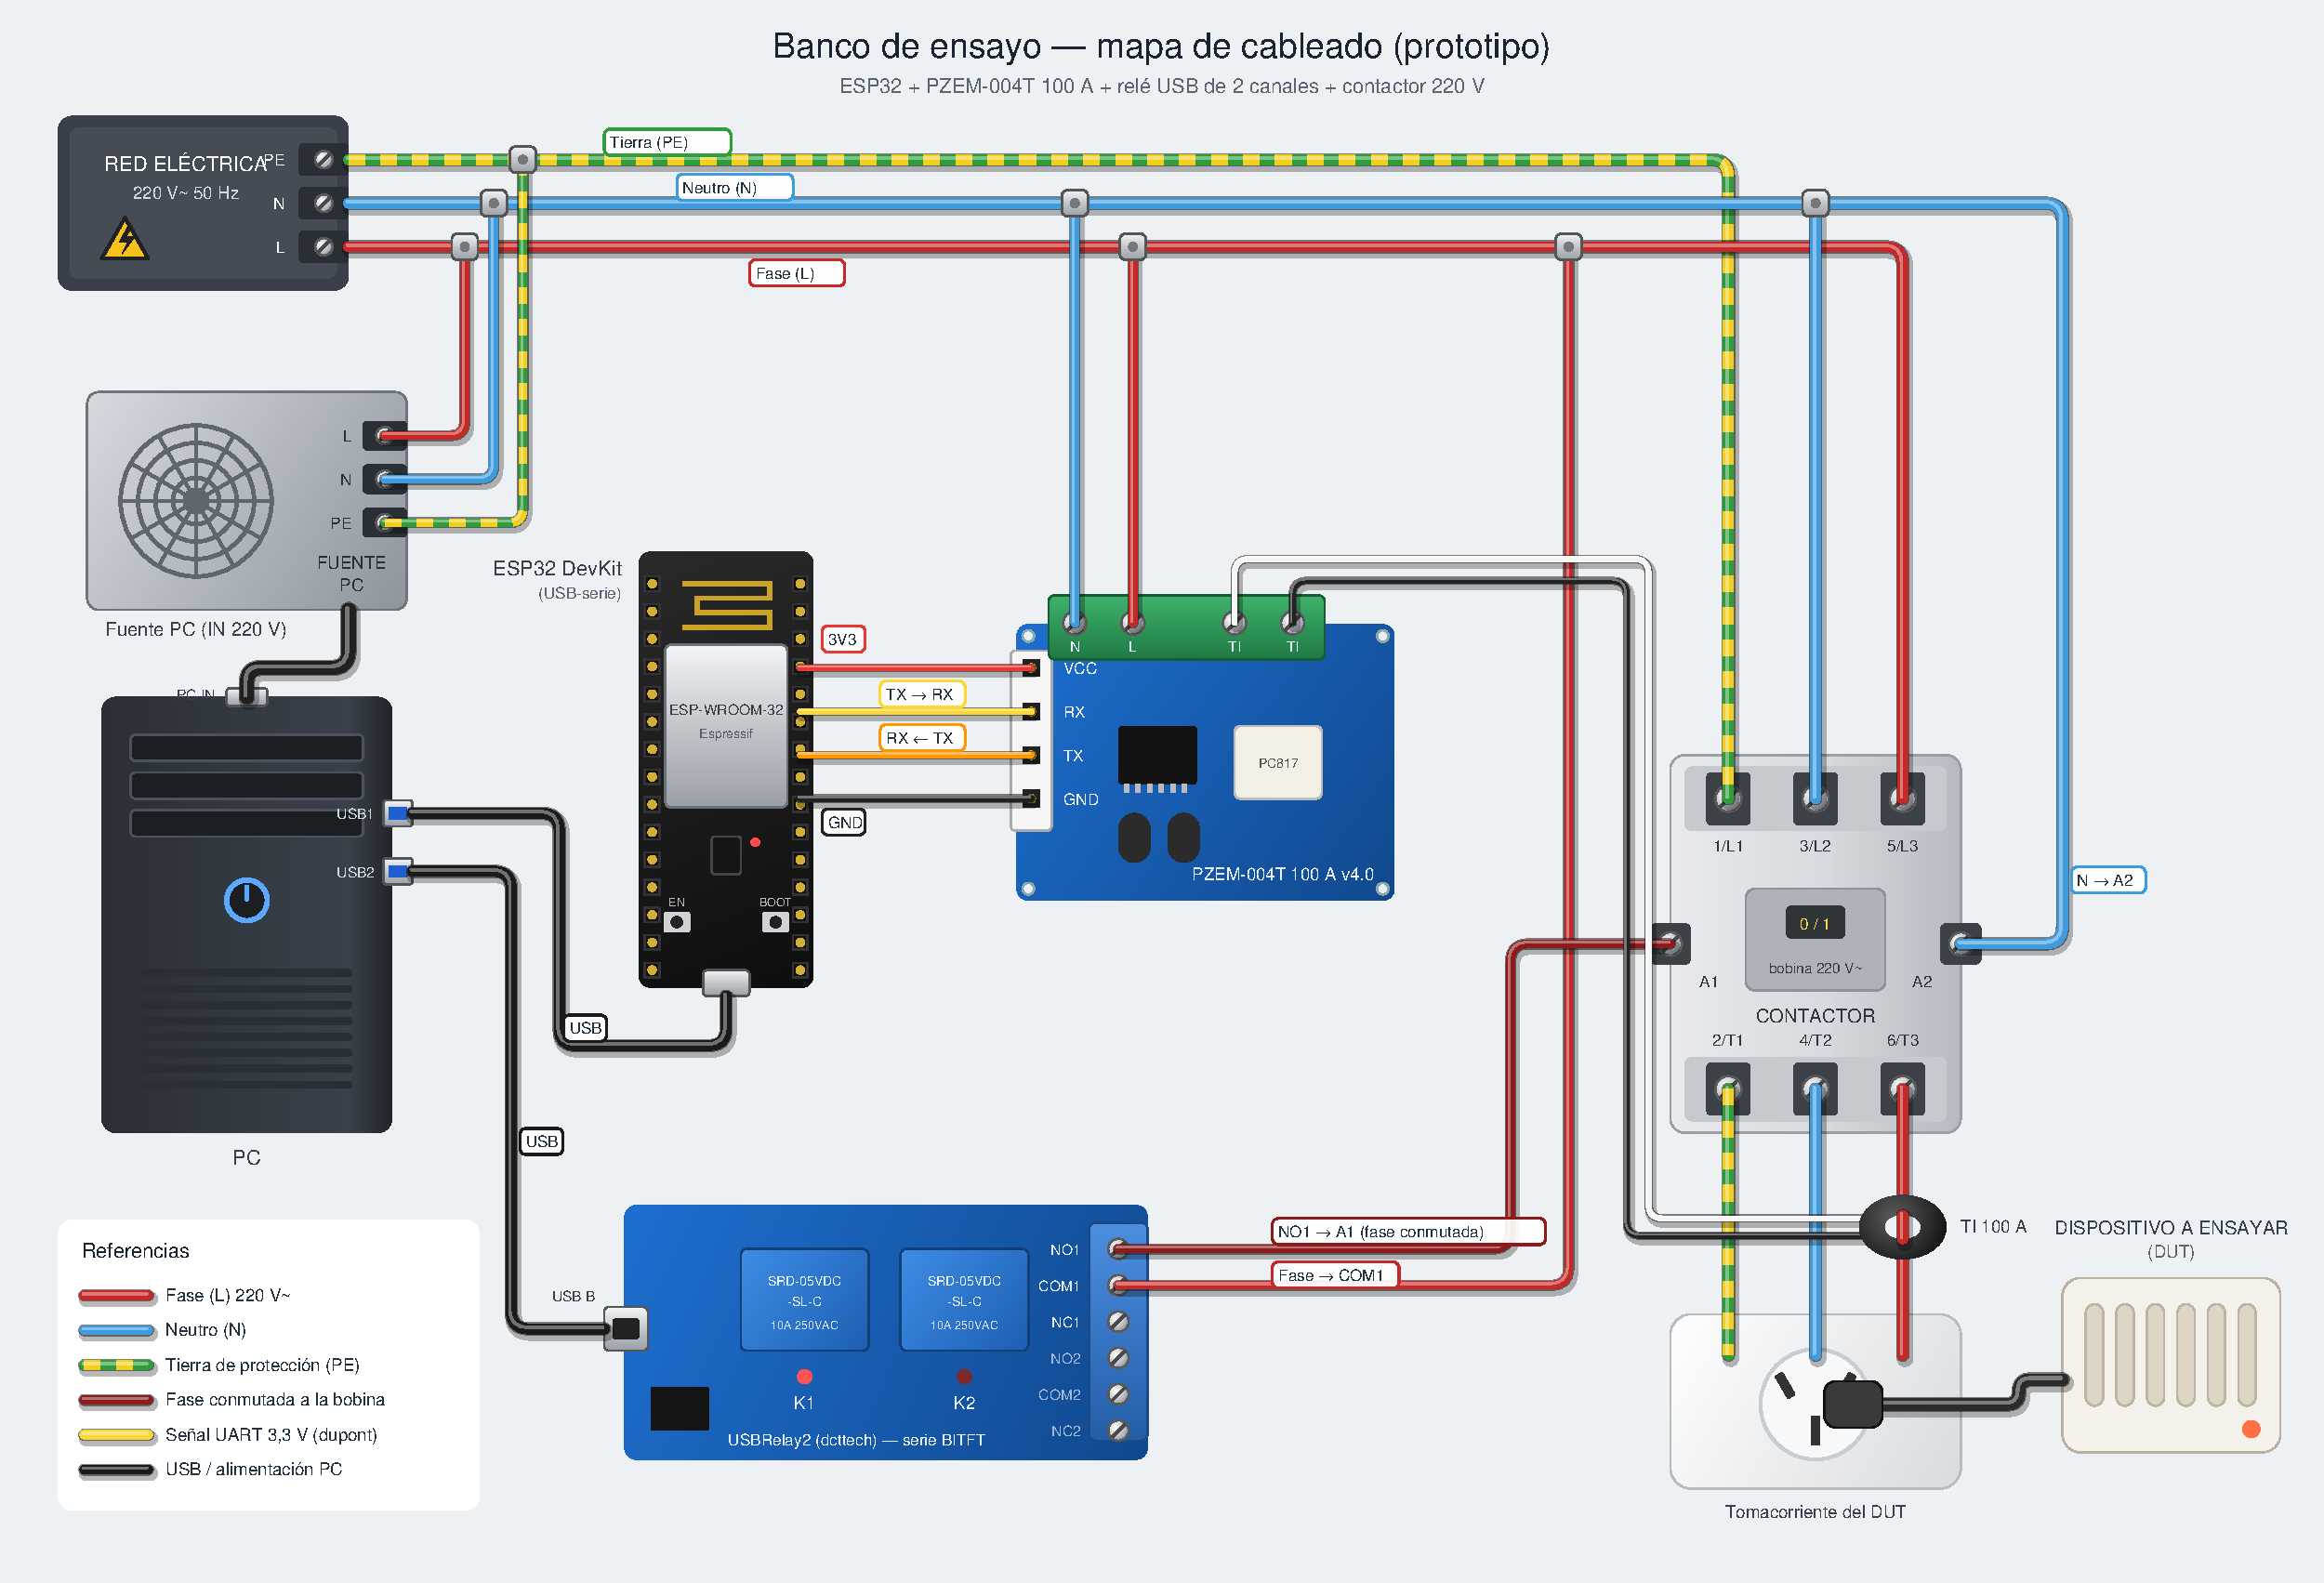
\includegraphics[width=\linewidth]{mapa_cableado.pdf}
    \caption{Versión ilustrada del esquema de cableado.}
    \label{fig:mapa_cableado}
\end{figure}

\subsection{Esquemas de conexión de los ensayos de seguridad}

Las Figuras~\ref{fig:conexion_fuga_activa} a~\ref{fig:conexion_pat} muestran el
\textbf{diseño propuesto} de conexión de los ensayos de seguridad, elaborado por
la autora a partir del equipo completo de SYGlab y de los requisitos de la norma.
No es hardware implementado en el prototipo propio: cada esquema indica la
secuencia que ejecuta el software y, en un recuadro, los puntos que quedan por
definir para construirlo (por ejemplo, la resolución del medidor para
\SI{0,75}{\milli\ampere} o la medición de la caída de tensión en puesta a
tierra).

\begin{figure}[htbp]
    \centering
    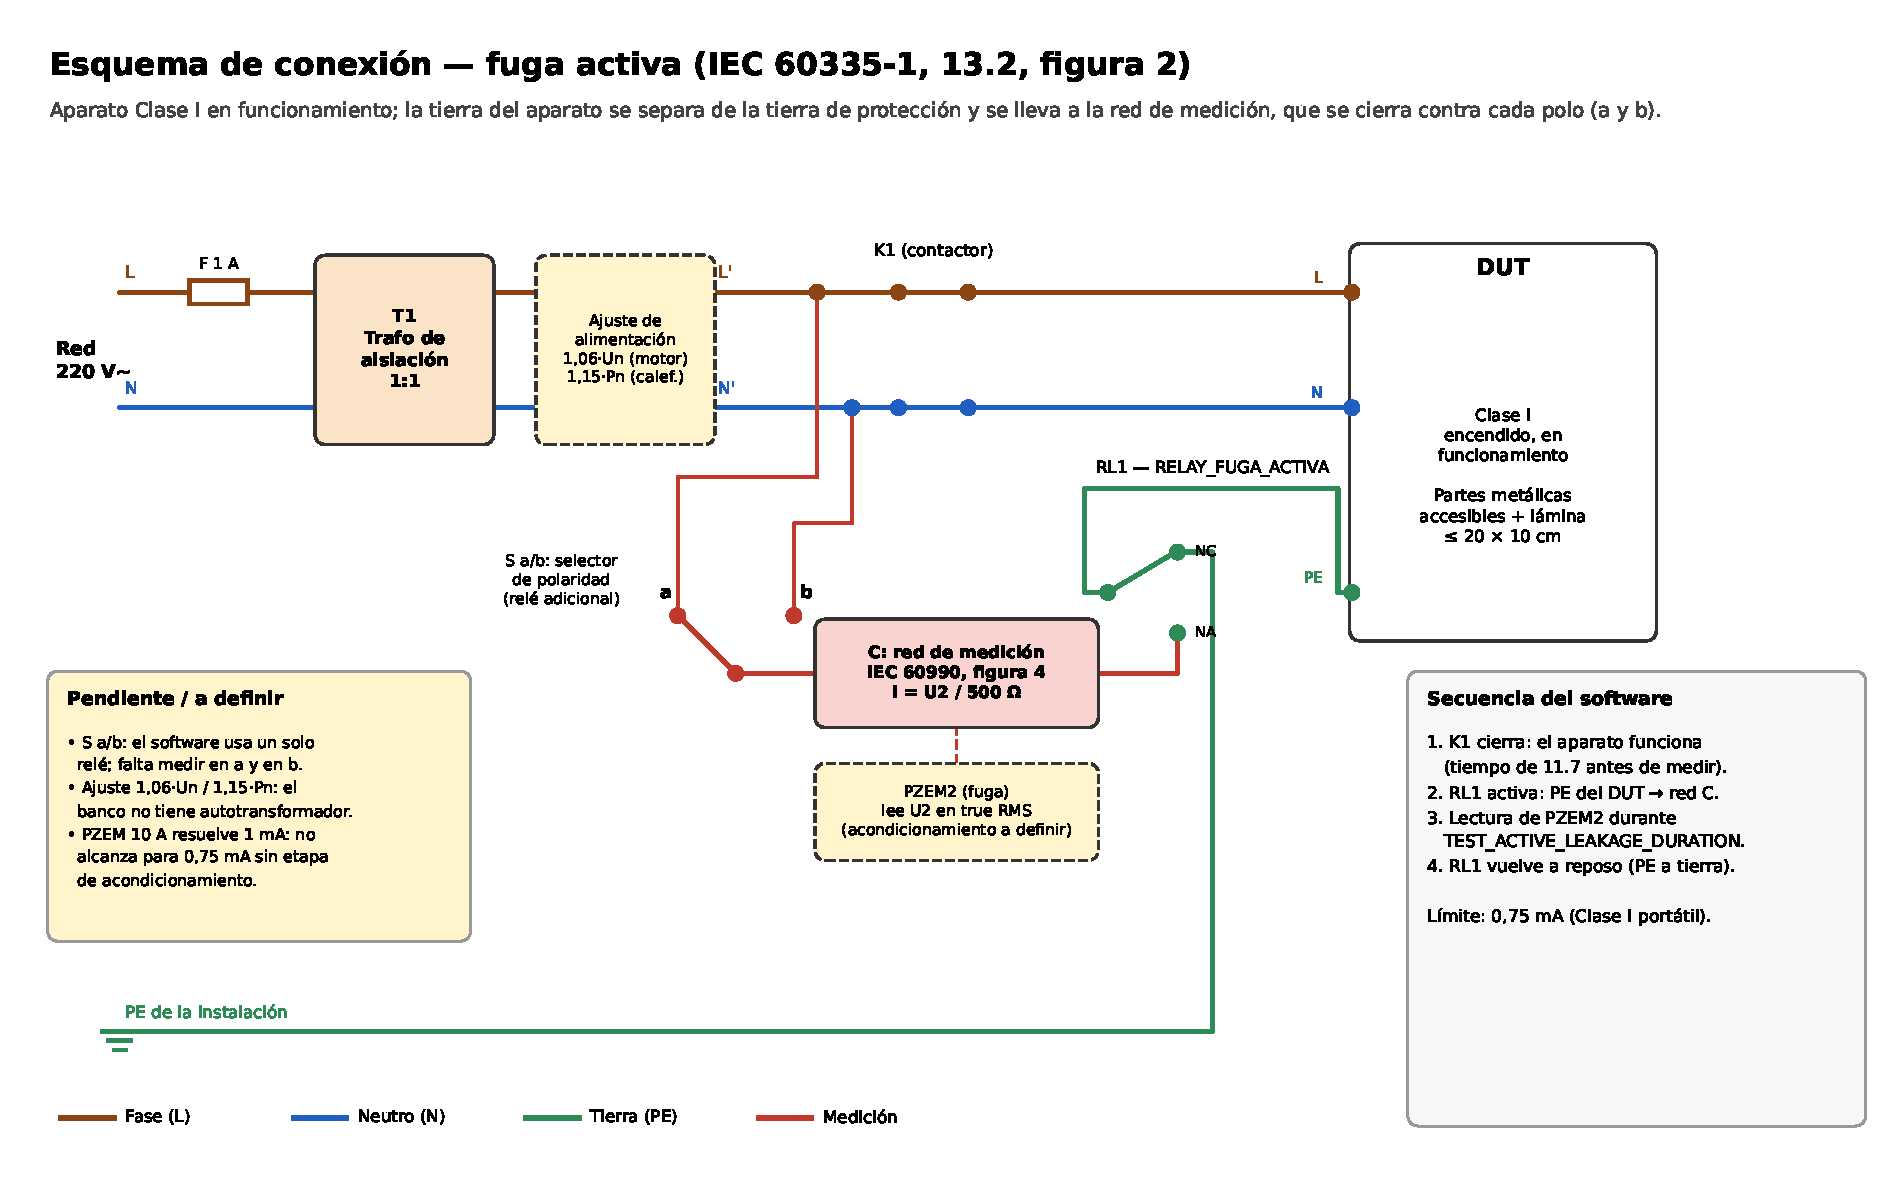
\includegraphics[width=\linewidth]{conexion_fuga_activa.pdf}
    \caption{Esquema de conexión del ensayo de fuga activa (IEC~60335-1, 13.2).}
    \label{fig:conexion_fuga_activa}
\end{figure}

\begin{figure}[htbp]
    \centering
    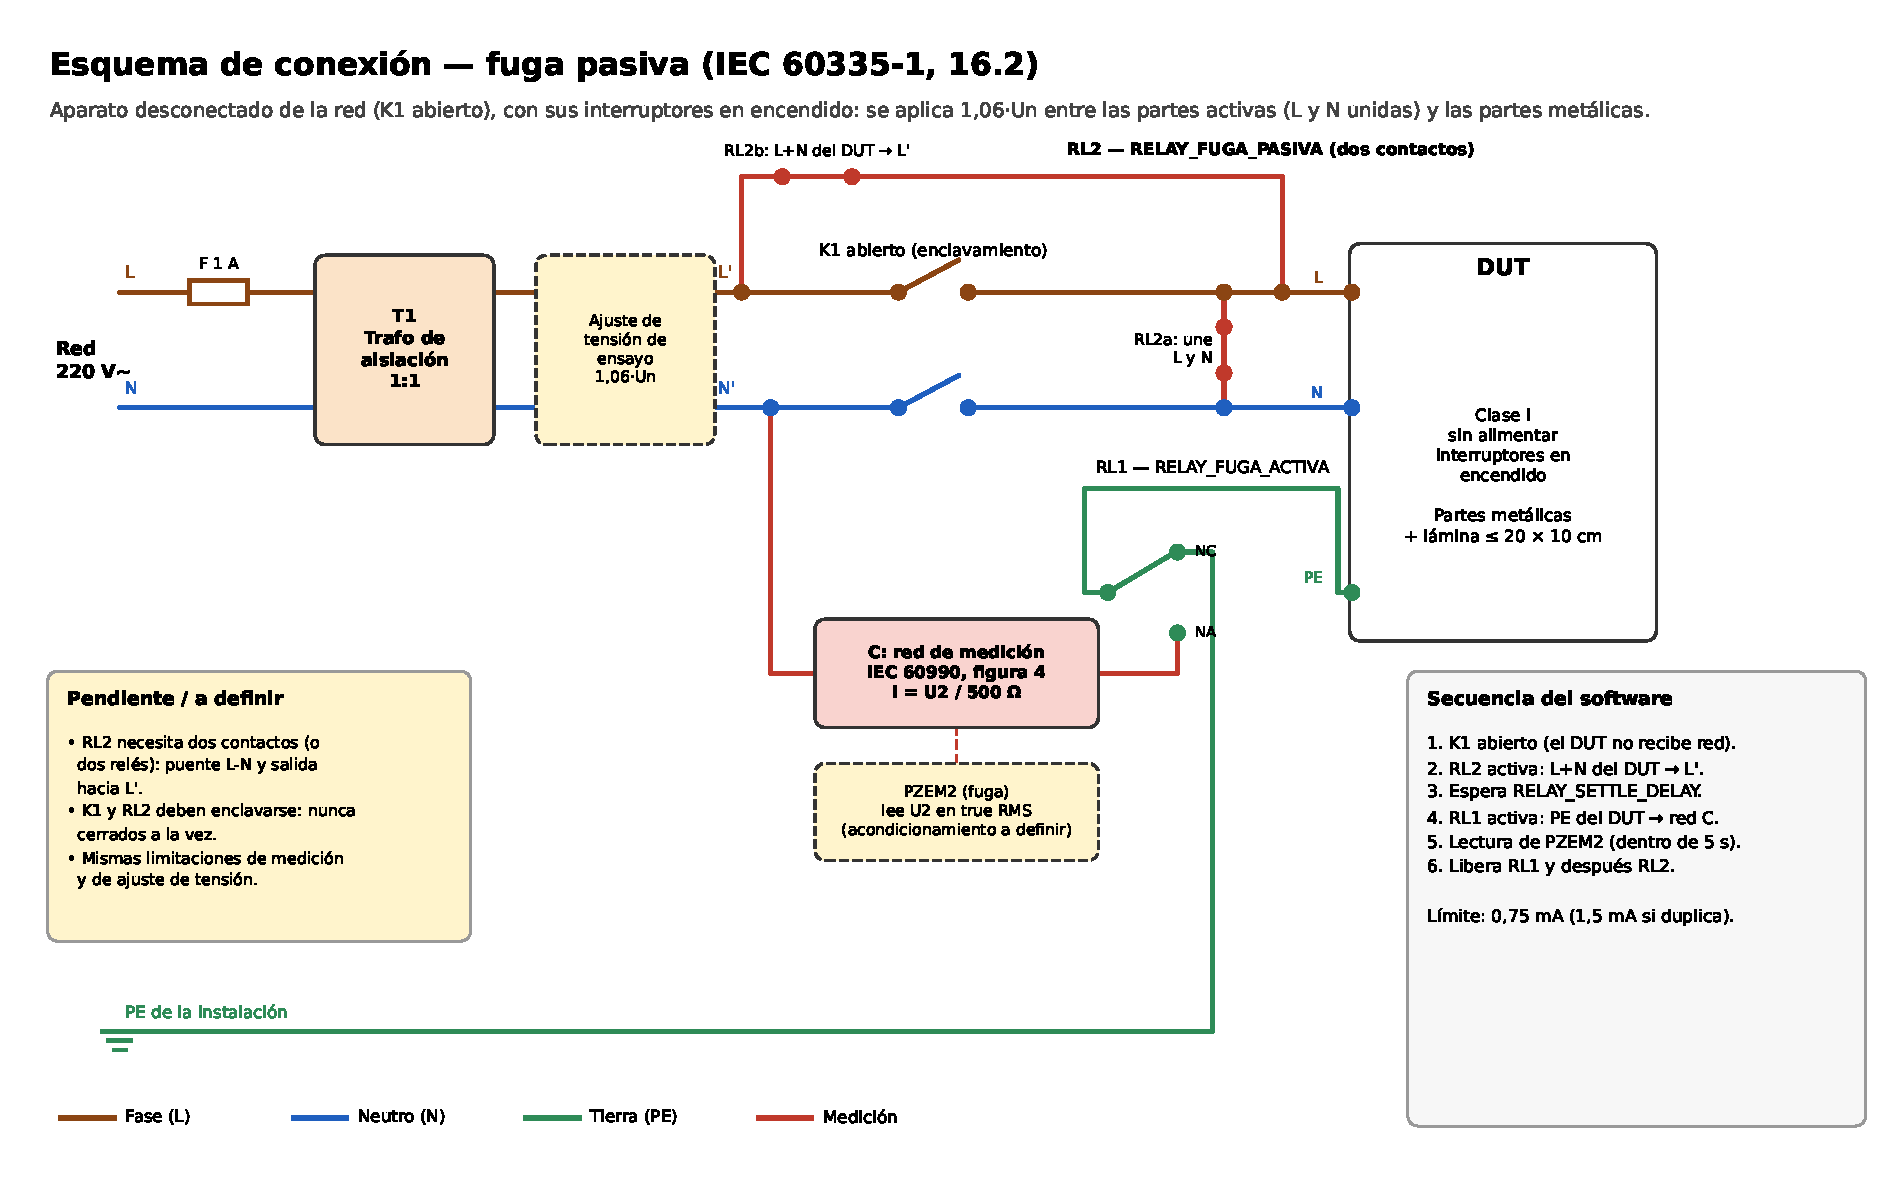
\includegraphics[width=\linewidth]{conexion_fuga_pasiva.pdf}
    \caption{Esquema de conexión del ensayo de fuga pasiva (IEC~60335-1, 16.2).}
    \label{fig:conexion_fuga_pasiva}
\end{figure}

\begin{figure}[htbp]
    \centering
    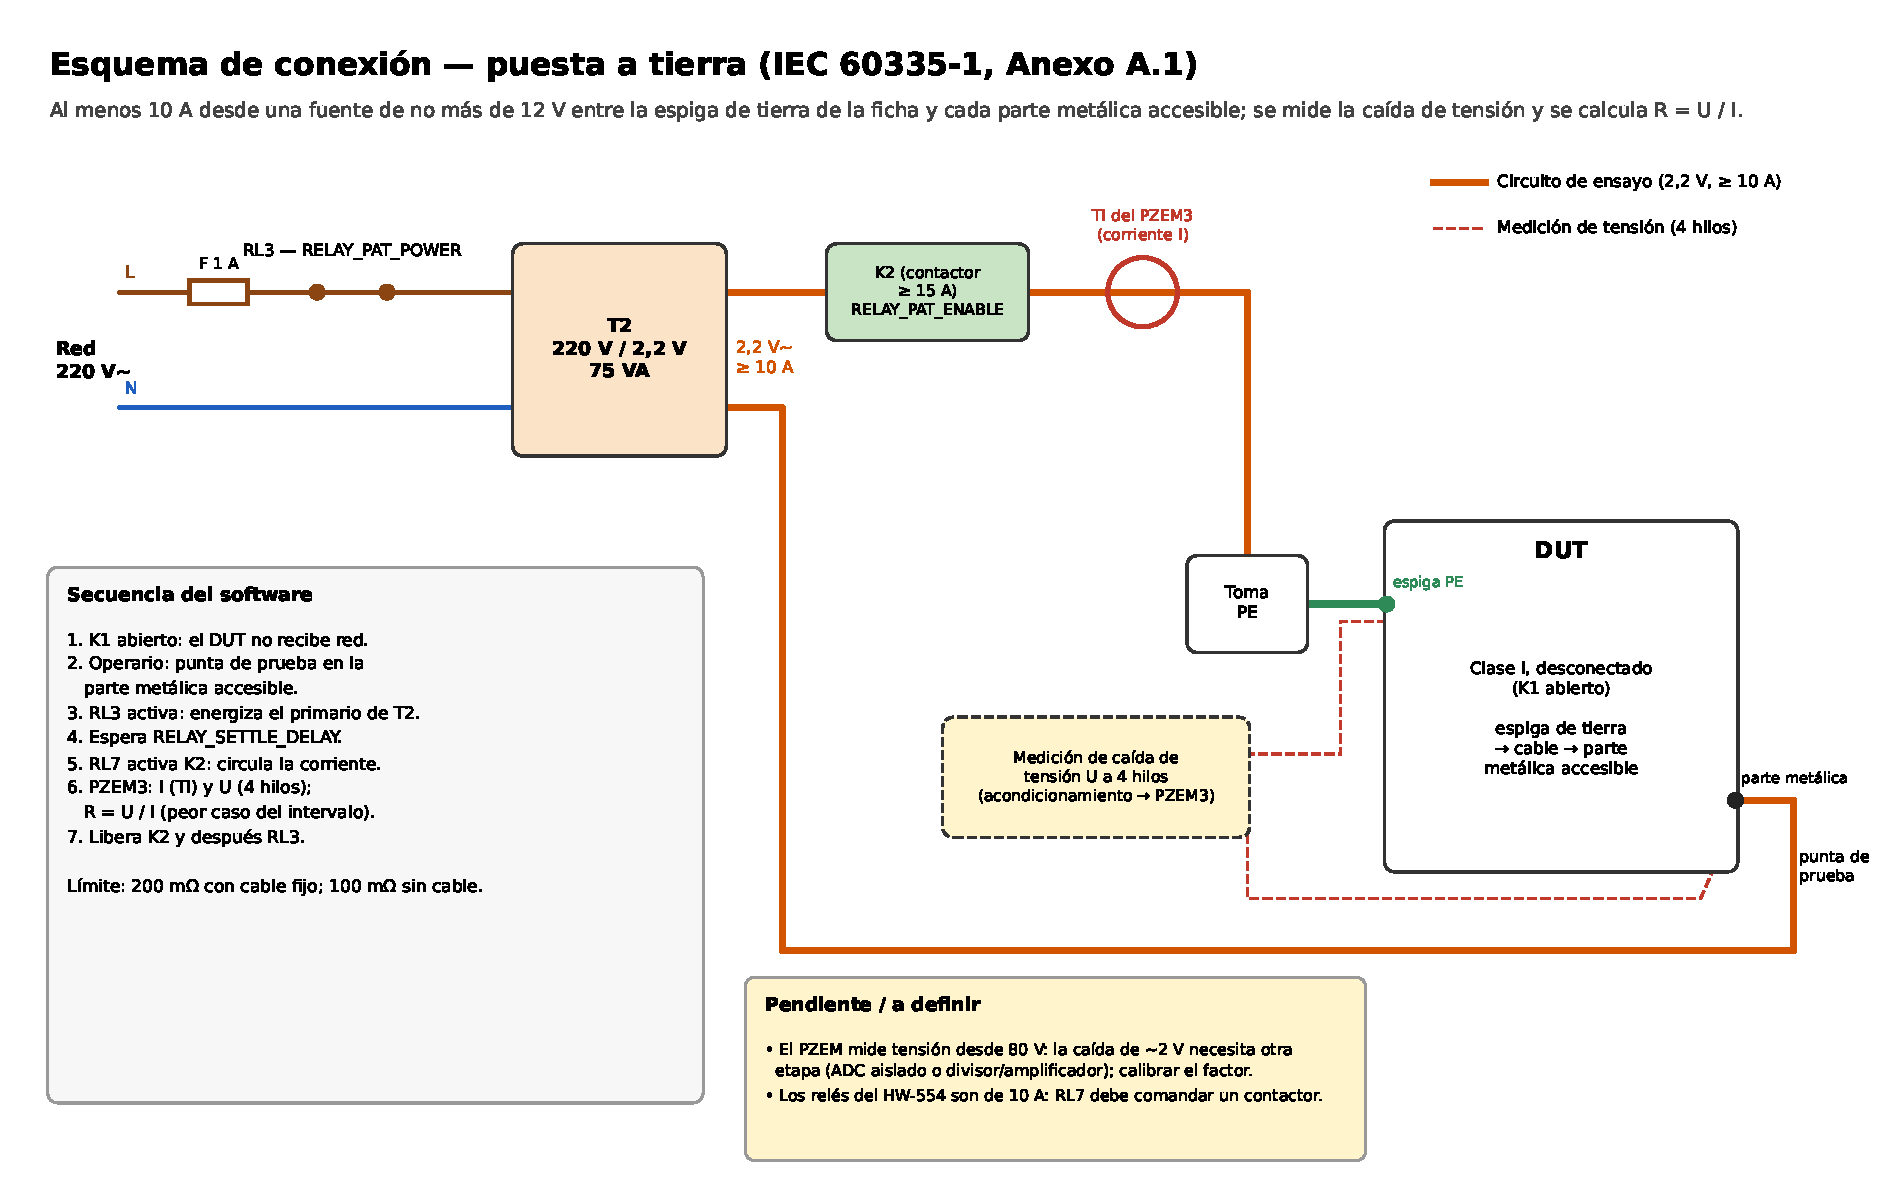
\includegraphics[width=\linewidth]{conexion_pat.pdf}
    \caption{Esquema de conexión del ensayo de puesta a tierra (IEC~60335-1,
             Anexo~A.1).}
    \label{fig:conexion_pat}
\end{figure}

\subsection{Fotografías}

La Figura~\ref{fig:equipo_completo} muestra el equipo completo de referencia
armado, con los contactores de cada ensayo (consumo, puesta a tierra y tensión
resistida de \SI{1}{\kilo\volt} y \SI{2,5}{\kilo\volt}), los transformadores de
ensayo, el módulo de relés y las borneras. La Figura~\ref{fig:banco_prototipo}
muestra el primer prototipo propio durante el ensayo de consumo del soldador.

\begin{figure}[htbp]
    \centering
    \begin{subfigure}[b]{0.66\linewidth}
        \centering
        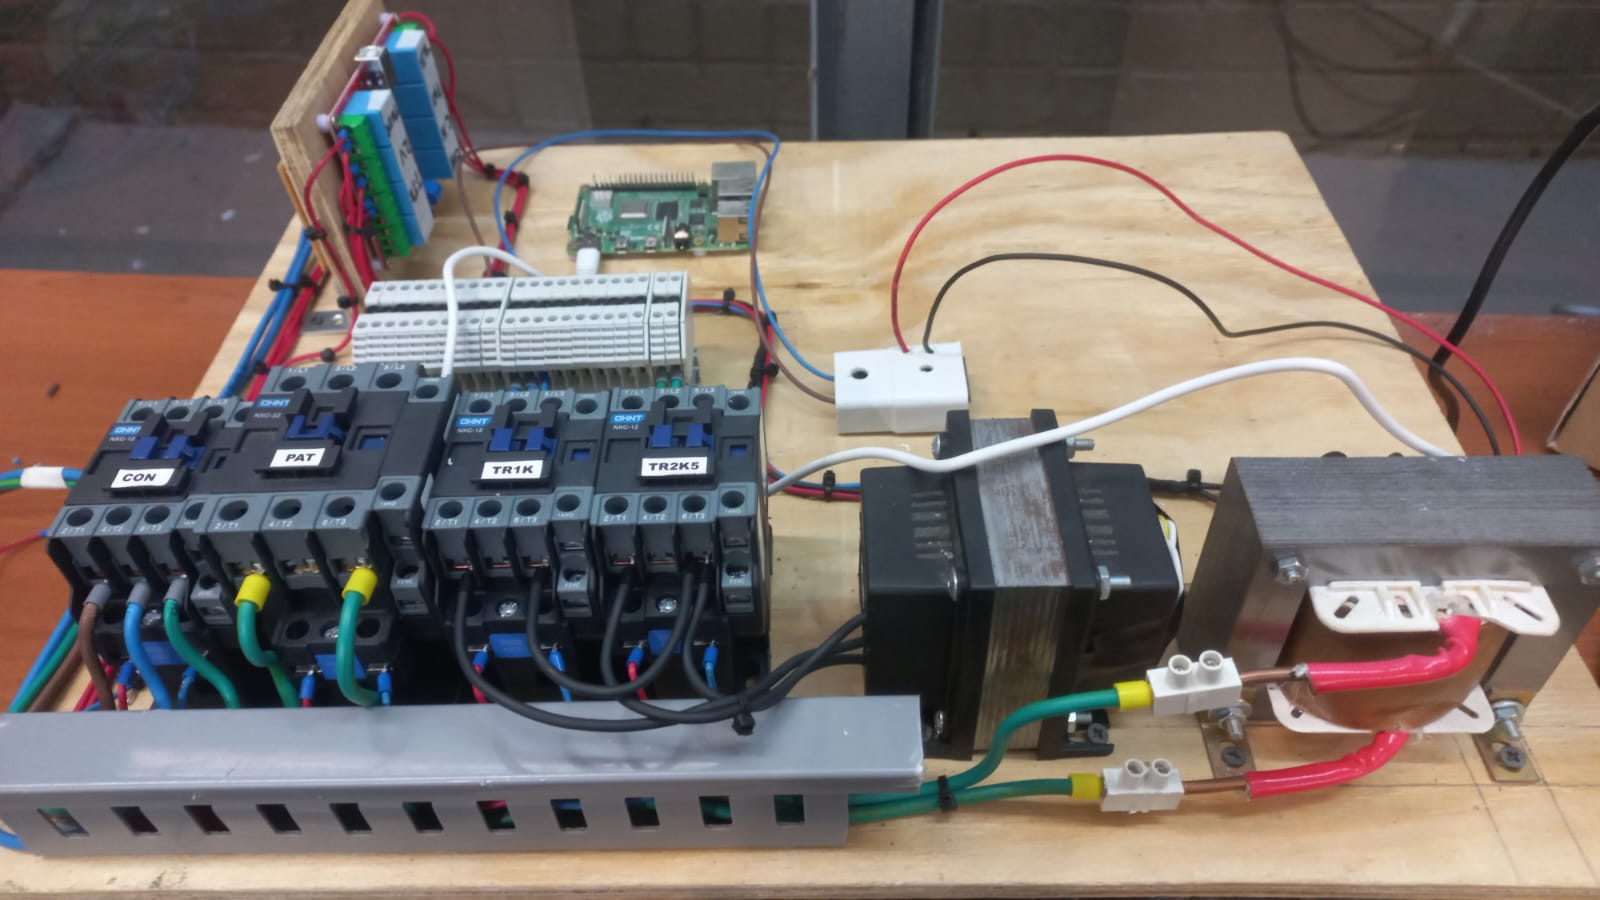
\includegraphics[height=5.8cm]{equipo_completo_general.jpg}
        \caption{Vista general.}
    \end{subfigure}\hfill
    \begin{subfigure}[b]{0.30\linewidth}
        \centering
        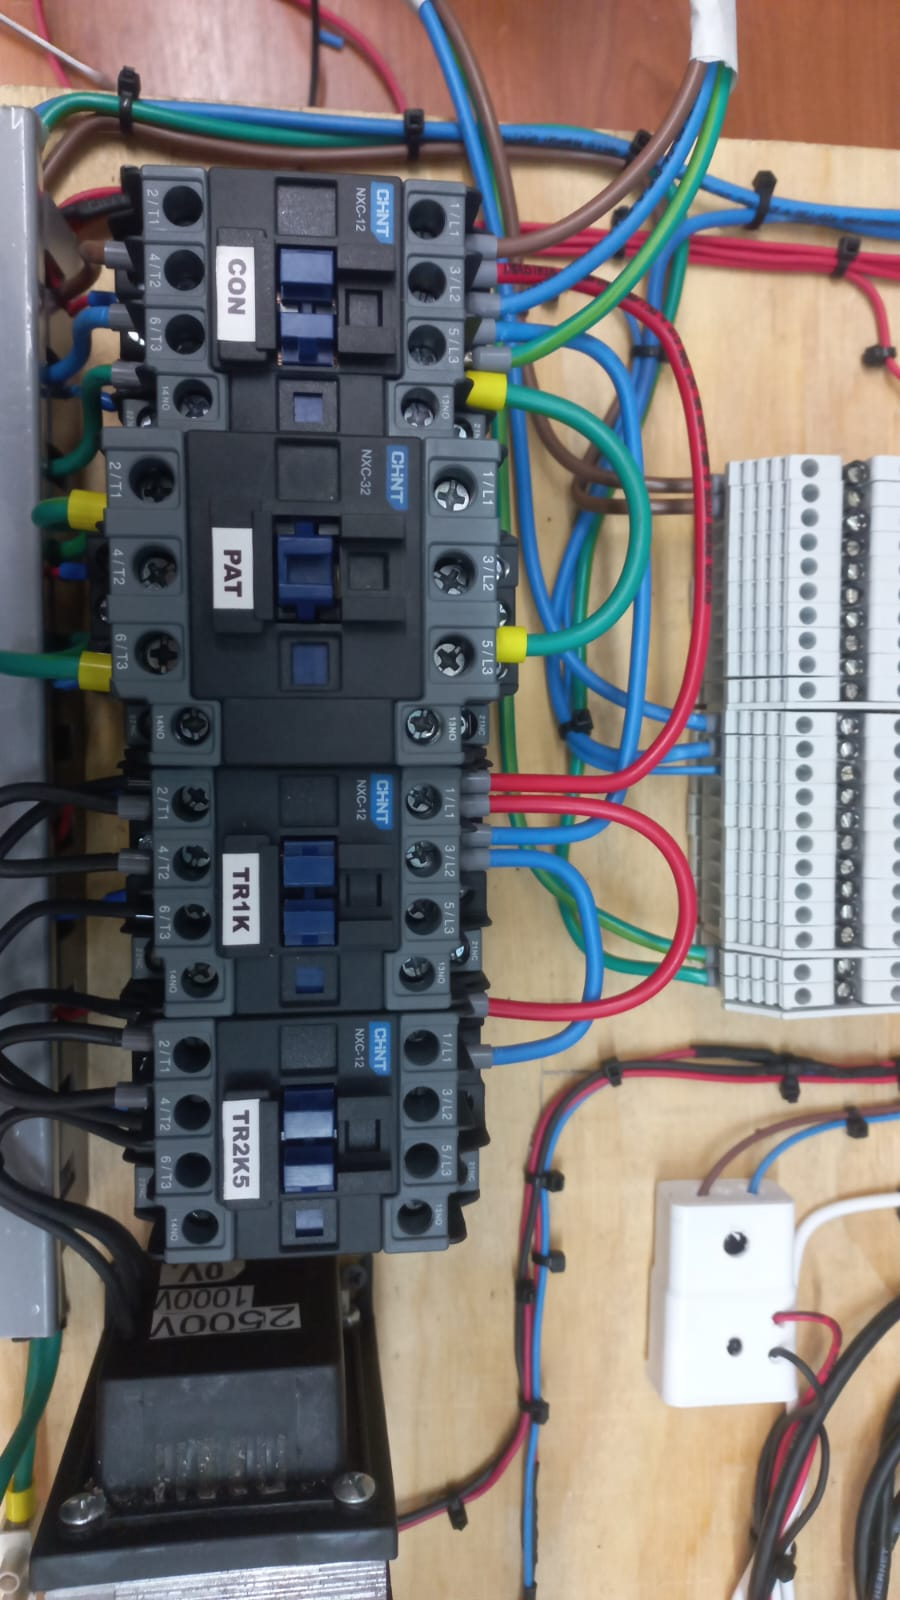
\includegraphics[height=6cm]{equipo_completo_contactores.jpg}
        \caption{Contactores de cada ensayo.}
    \end{subfigure}
    \caption{Equipo completo de referencia armado.}
    \label{fig:equipo_completo}
\end{figure}

\begin{figure}[htbp]
    \centering
    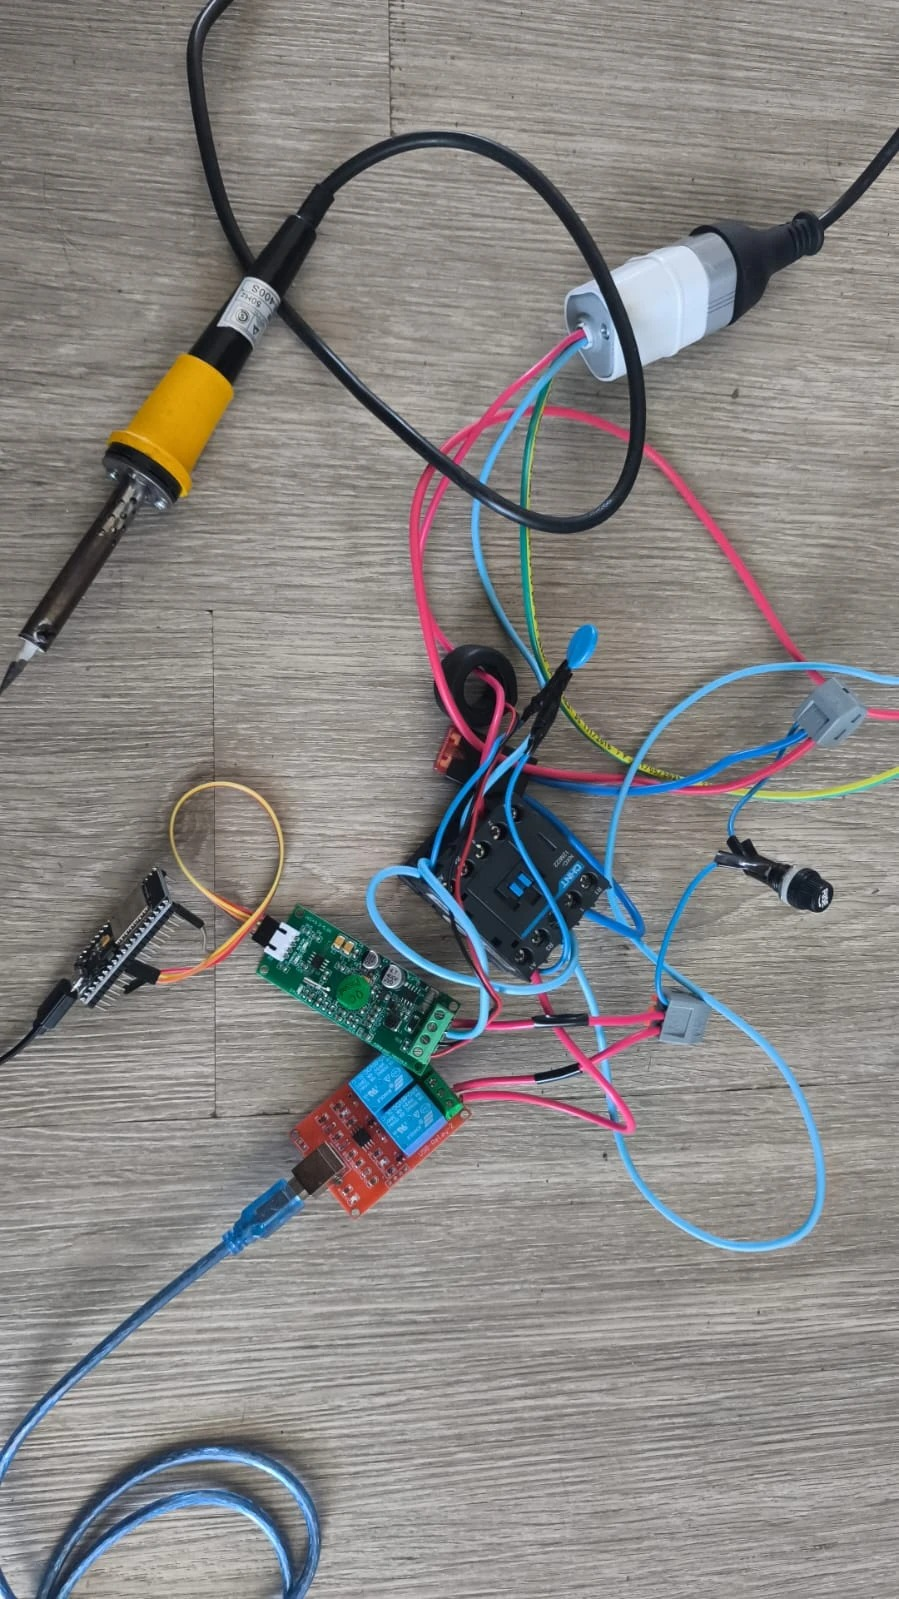
\includegraphics[height=0.6\textheight,keepaspectratio]{banco_prototipo_soldador.jpg}
    \caption{Primer prototipo propio (ESP32, PZEM-004T, placa de relés USB y
             contactor) durante el ensayo de consumo del soldador.}
    \label{fig:banco_prototipo}
\end{figure}

\subsection{Registro de hallazgos}

La Tabla~\ref{tab:hallazgos} resume los hallazgos principales y su resolución.

\begin{longtable}{@{} p{4.2cm} p{5.3cm} p{5.3cm} @{}}
\caption{Hallazgos principales y su resolución}\label{tab:hallazgos}\\
\toprule
\textbf{Hallazgo} & \textbf{Causa} & \textbf{Resolución} \\
\midrule
\endfirsthead
\toprule
\textbf{Hallazgo} & \textbf{Causa} & \textbf{Resolución} \\
\midrule
\endhead
\multicolumn{3}{@{}l}{\textit{Normativos}} \\
Rigidez evaluada solo por tensión
  & Se tomó la corriente de la fuente como límite de aprobación
  & Criterio del Anexo~A.2: corriente $\leq$ \SI{5}{\milli\ampere} con la
    tensión de ensayo aplicada \\
Fuga pasiva con límite fijo de \SI{1500}{\micro\ampere}
  & Se usaba siempre el límite duplicado
  & \SI{750}{\micro\ampere}; \SI{1500}{\micro\ampere} solo con condición de
    duplicación (16.2) \\
Puesta a tierra con límite único
  & Sin distinguir cable fijo ni controlar la corriente
  & \SI{200}{\milli\ohm} o \SI{100}{\milli\ohm} con corriente
    $\geq$ \SI{10}{\ampere} (A.1) \\
Consumo con porcentajes fijos
  & Tolerancia única para todos los aparatos
  & Tablas~1 y~2 según tipo y potencia nominal \\
\midrule
\multicolumn{3}{@{}l}{\textit{Hardware}} \\
ESP32 no detectado
  & Cable USB solo de carga; faltaba el controlador CP210x
  & Cambio de cable e instalación del controlador \\
ESP32 no respondía
  & Firmware de fábrica (comandos AT)
  & Firmware propio \\
Bucle de arranque del ESP32
  & Medidor en el puerto del USB y alimentado con \SI{5}{\volt}
  & Medidor en GPIO16/17 alimentado con \SI{3,3}{\volt} \\
Bornes del medidor sin identificar
  & Bornera sin serigrafía
  & Identificación por resistencia con multímetro \\
Desconexión de la placa de relés
  & Interferencia al abrir el contactor con carga con motor
  & Software tolerante con falla segura y varistor en la bobina (mitigado) \\
Medidor sin resolución para fuga
  & Umbral de arranque de unos \SI{20}{\milli\ampere}
  & Requiere versión de \SI{10}{\ampere} y red IEC~60990 (pendiente) \\
\midrule
\multicolumn{3}{@{}l}{\textit{Software}} \\
Interfaz sin lógica
  & Ventana principal en estado de esqueleto
  & Integración de las ocho pestañas \\
Integración continua sin pruebas
  & Configuración sin las dependencias de desarrollo
  & Flujo corregido; 62 errores de estilo resueltos \\
Correcciones de calibración sin efecto
  & Nunca se aplicaban a las lecturas
  & Aplicadas a todas las lecturas \\
Consumo subestimado \SI{27}{\percent}
  & Lecturas del transitorio de cierre en el promedio
  & Descarte de lecturas de estabilización \\
Credenciales de fábrica en la API
  & Contraseña en texto plano
  & Hash PBKDF2-SHA256 y rechazo de credenciales de fábrica \\
Fuga sin medidor: NO EJECUTADO
  & Lectura fallida sin veredicto
  & Lectura fallida = FALLA en ensayos de seguridad \\
\bottomrule
\end{longtable}

\subsection{Datos y scripts}

\begin{itemize}
    \item Base de datos de la prueba de punta a punta (16 ensayos y 10 muestras de perfil de consumo).
    \item Exportación a Excel generada por la aplicación.
    \item Cuaderno de comandos con las lecturas directas del ventilador y del
          soldador.
    \item Scripts de prueba que operan la aplicación real con el
          hardware real.
\end{itemize}

\end{appendices}

\end{document}
